% !TEX program = pdflatex
% !TEX encoding = UTF-8 Unicode

% Plantilla de la clase `scrbook` del paquete KOMA-script para la
% elaboración de un TFG siguiendo las directrices del la comisión del
% Grado en Matemáticas de la Universidad de Granada.

% Francisco Torralbo Torralbo
% miércoles, 29 de abril de 2020

\documentclass{scrbook}

\KOMAoptions{%
  fontsize=10pt,        % Tamaño de fuente
  paper=a4,             % Tamaño del papel
  headings=normal,      % Tamaño de letra para los títulos: small, normal, big
  % parskip=half,         % Espacio entre párrafos: full (una línea) o half (media línea)
  headsepline=false,    % Una linea separa la cabecera del texto
  cleardoublepage=empty,% No imprime cabecera ni pie en páginas en blanco 
  chapterprefix=false,  % No antepone el texto "capítulo" antes del número
  appendixprefix=false,	% No antepone el texto "Apéndice" antes de la letra
  listof=totoc,		    	% Añade a la tabla de contenidos la lista de tablas y figuras
  index=totoc,			    % Añade a la talba de contenidos una entrada para el índice
  bibliography=totoc,	  % Añade a la tabla de contenidos una entrada para bibliografía
  BCOR=5mm,           % Reserva margen interior para la encuadernación. 
                        % El valor dependerá el tipo de encuadernado y del grosor del libro.
  DIV=10,             % Cálcula el diseño de página según ciertos 
                        % parámetros. Al aumentar el número aumentamos el ancho de texto y disminuimos el ancho del margen. Una opción de 14 producirá márgenes estrechos y texto ancho.
}

% INFORMACIÓN PARA LA VERSIÓN IMPRESA
% Si el documento ha de ser impreso en papel de tamaño a4 pero el tamaño del documento (elegido en \KOMAoptions con la ocpión paper) no es a4 descomentar la línea que carga el paquete `crop` más abajo. El paquete crop se encargará de centrar el documento en un a4 e imprimir unas guías de corte. El procedimiento completo para imprenta sería el siguiente:
% 0. Determinar, según el tipo de encuadernación del documento, el ancho reservado para el proceso de encuadernación (preguntar en la imprenta), es decir, la anchura del área del papel que se pierde durante el proceso de encuadernación. Fijar la varibale BCOR de \KOMAoptions a dicho valor.
% 1. Descomentar la siguiente línea e imprimir una única página con las guías de corte
% 2. Cambiar la opción `cross` por `cam` (o `off`) en el paquete crop y volver a compilar. Imprimir el documento (las guías de corte impresas no inferfieren con el texto).
% 3. Usar la página con las guías impresas en el punto 1 para cortar todas las páginas.

% \usepackage[a4, odd, center, pdflatex, cross]{crop} % Permite imprimir el documento en un a4 (si el tamaño es más pequeño) mostrando unas guías de corte. Útil para imprenta.

% VERSIÓN ELECTRÓNICA PARA TABLETA
% Las opciones siguientes seleccionan un tamaño de impresión similar a una tableta de 9 pulgadas con márgenes estrechos. Útil para producir una versión en pdf para ser leída en una tableta en lugar de impresa.
% Para que la portada quede centrada correctamente hay que editar el
% archivo `portada.tex` y eliminar el entorno `addmargin`

% \KOMAoptions{fontsize=10pt, paper=19.7104cm:14.7828cm, twoside=false, BCOR=0cm, DIV=14}

% ---------------------------------------------------------------------
%	PAQUETES 
% ---------------------------------------------------------------------

% CODIFICACIÓN E IDIOMA
% ---------------------------------------------------------------------
\usepackage[utf8]{inputenc} 			    % Codificación de caracteres

% Selección del idioma: cargamos por defecto inglés y español (aunque este último es el idioma por defecto para el documento). Cuando queramos cambiar de idioma escribiremos:
% \selectlanguage{english} o \selectlanguage{spanish}

\usepackage[english, spanish, es-nodecimaldot, es-noindentfirst, es-tabla]{babel}

% Opciones cargadas para el paquete babel:
  % es-nodecimaldot: No cambia el punto decimal por una coma en modo matemático.
  % es-noindentfirst: No sangra los párrafos tras los títulos.
  % es-tabla: cambia el título del entorno `table` de "Cuadro" a "Tabla"

% Otras opciones del paquete spanish-babel:
  \unaccentedoperators % Desactiva los acentos en los operadores matemáticso (p.e. \lim, \max, ...). Eliminar esta opción si queremos que vayan acentuados

% MATEMÁTICAS
% ---------------------------------------------------------------------
\usepackage{amsmath, amsthm, amssymb} % Paquetes matemáticas
\usepackage{mathtools}                % Añade mejoras a amsmath
\mathtoolsset{showonlyrefs=true}      % sólo se numeran las ecuaciones que se usan
\usepackage[mathscr]{eucal} 					% Proporciona el comando \mathscr para
                                      % fuentes de tipo manuscrito en modo matemático sin sobreescribir el comando \mathcalE
% TIPOGRAFÍA 
% ---------------------------------------------------------------------
% El paquete microtype mejora la tipografía del documento.
\usepackage[activate={true,nocompatibility},final,tracking=true,kerning=true,spacing=true,factor=1100,stretch=10,shrink=10]{microtype}

% Para modificar el tamaño de la fuente dentro de las ecuaciones
\usepackage{scalerel}

% Las tipografías elegidas para el documento, siguiendo la guía de estilo de la UGR,
% son las siguientes
% Normal font: 			URW Palladio typeface. 
% Sans-serif font: 	Gill Sans
% Monospace font: 	Inconsolata
\usepackage[T1]{fontenc}
\usepackage[sc, osf]{mathpazo} \linespread{1.05}         
\usepackage[scaled=.95,type1]{cabin} % sans serif in style of Gill Sans
% Si el paquete cabin da error usar el siguiente comando en su lugar
% \renewcommand{\sfdefault}{iwona} 
\usepackage{inconsolata}


% Selecciona el tipo de fuente para los títulos (capítulo, sección, subsección) del documento.
\setkomafont{disposition}{\sffamily\bfseries}

% Cambia el ancho de la cita. Al inicio de un capítulo podemos usar el comando \dictum[autor]{cita} para añadir una cita famosa de un autor.
\renewcommand{\dictumwidth}{0.45\textwidth} 

\recalctypearea % Necesario tras definir la tipografía a usar.

\usepackage{setspace}
% TABLAS, GRÁFICOS Y LISTADOS DE CÓDIGO
% ---------------------------------------------------------------------
\usepackage{booktabs}
% \renewcommand{\arraystretch}{1.5} % Aumenta el espacio vertical entre las filas de un entorno tabular

\usepackage{xcolor, graphicx}
% Carpeta donde buscar los archivos de imagen por defecto
\graphicspath{{img/}}

% IMAGEN DE LA PORTADA
% Existen varias opciones para la imagen de fondo de la portada del TFG. Todas ellas tienen en logotipo de la universidad de Granada en la cabecera. Las opciones son las siguientes:
% 1. portada-ugr y portada-ugr-color: diseño con marca de agua basada en el logo de la UGR (en escala de grises y color).
% 2. portada-ugr-sencilla y portada-ugr-sencilla-color: portada únicamente con el logotipo de la UGR en la cabecera.
\usepackage{eso-pic}
\newcommand\BackgroundPic{%
	\put(0,0){%
		\parbox[b][\paperheight]{\paperwidth}{%
			\vfill
			\centering
      % Indicar la imagen de fondo en el siguiente comando
			
\includegraphics[width=\paperwidth,height=\paperheight,%
			keepaspectratio]{portada-ugr-sencilla}%
			\vfill
}}}

% \usepackage{listings} % Para la inclusión de trozos de código

% CABECERAS
% ---------------------------------------------------------------------
% Si queremos modificar las cabeceras del documento podemos usar el paquete
% `scrlayer-scrpage` de KOMA-Script. Consultar la documentación al respecto.
% \usepackage[automark]{scrlayer-scrpage}

% VARIOS
% ---------------------------------------------------------------------

%\usepackage{showkeys}	% Muestra las etiquetas del documento. Útil para revisar las referencias cruzadas.

% ÍNDICE 
% Para generar el índice hay que compilar el documento con MakeIndex. Generalmente los editores se encargan de ello automáticamente.
% ----------------------------------------------------------------------
% \index{} para añadir un elemento
% \index{main!sub} para añadir un elementos "sub" bajo la categoría "main".
% \index{termino|textbf} para dar formato al número de página (negrita).
% \index{termino|see{termino relacionado}} para crear una referencia cruzada

% Ejemplo: \index{espacio homogéneo}, \index{superficie!mínima}, \index{esfera|see{espacio homogéneo}}

% Activar los siguientes comandos para generar el índice terminológico. Ver también comandos al final de este documento para incluir dicho índice en el pdf final.
% \usepackage{makeidx}
% \makeindex

% Para revisar las entradas al índice conforme las incluimos en el documento es útil el siguiente paquete. Conviene observar que mientras esté cargado no se generará el índice.
%\usepackage{showidx} % Muestra en el margen del documento las entradas añadidas al índice. Útil para revisar el documento. Si está activo el índice no se genera

% ---------------------------------------------------------------------
% COMANDOS Y ENTORNOS
% ---------------------------------------------------------------------
% Cargamos un archivo externo donde hemos incluido todos los comandos
% propios que vamos a usar en el documento.
% DEFINICIÓN DE COMANDOS Y ENTORNOS

% CONJUNTOS DE NÚMEROS

  \newcommand{\N}{\mathbb{N}}     % Naturales
  \newcommand{\R}{\mathbb{R}}     % Reales
  \newcommand{\Z}{\mathbb{Z}}     % Enteros
  \newcommand{\Q}{\mathbb{Q}}     % Racionales
  \newcommand{\C}{\mathbb{C}}     % Complejos

% TEOREMAS Y ENTORNOS ASOCIADOS

  % \newtheorem{theorem}{Theorem}[chapter]
  \newtheorem*{teorema*}{Teorema}
  \newtheorem{teorema}{Teorema}[chapter]
  \newtheorem{proposicion}{Proposición}[chapter]
  \newtheorem{lema}{Lema}[chapter]
  \newtheorem{corolario}{Corolario}[chapter]

    \theoremstyle{definition}
  \newtheorem{definicion}{Definición}[chapter]
  \newtheorem{ejemplo}{Ejemplo}[chapter]

    \theoremstyle{remark}
  \newtheorem{observacion}{Observación}[chapter]
 
 \makeatletter
 \renewcommand*\env@matrix[1][\arraystretch]{%
 	\edef\arraystretch{#1}%
 	\hskip -\arraycolsep
 	\let\@ifnextchar\new@ifnextchar
 	\array{*\c@MaxMatrixCols c}}
 \makeatother

\newcommand{\shorteqnote}[1]{ & \text{\small\llap{#1}}}

% --------------------------------------------------------------------
% INFORMACIÓN DEL TFG Y EL AUTOR
% --------------------------------------------------------------------
\usepackage{xspace} % Para problemas de espaciado al definir comandos

\newcommand{\miTitulo}{Métodos para la resolución de ecuaciones integrales y su integración en un sistema para la simulación de la distribución de temperatura en edificios mediante el uso de servicios\xspace}
\newcommand{\miNombre}{David Cantón Ruiz\xspace}
\newcommand{\miGrado}{Doble Grado en Ingeniería Informática y Matemáticas}
\newcommand{\miFacultad}{Facultad de Ciencias	\\ Escuela Técnica Superior de Ingenierías Informática y de Telecomunicación}
\newcommand{\miUniversidad}{Universidad de Granada}
% Añadir tantos tutores como sea necesario separando cada uno de ellos
% mediante el comando `\medskip` y una línea en blanco
\newcommand{\miTutor}{
  Manuel Ruiz Galán \\ \emph{Departamento de Matemática Aplicada} 

  % Añadir tantos tutores como sea necesario. 

  \medskip
  Ángel Ruiz Zafra \\ \emph{Departamento de Lenguajes y Sistemas Informáticos}
}
\newcommand{\miCurso}{2023-2024\xspace}

% HYPERREFERENCES
% --------------------------------------------------------------------
\usepackage{xurl}
\usepackage{hyperref}
% Opciones para el paquete hyperref
%----------------------------------

\hypersetup{%
  % hidelinks,            % Enlaces sin color ni borde. El borde no se imprime
  linkbordercolor=0.8 0 0,
  citebordercolor=0 0.8 0,
  citebordercolor=0 0.8 0,
  colorlinks = true,            % Color en texto de los enlaces. Comentar esta línea o cambiar `true` por `false` para imprimir el documento.
  linkcolor = [rgb]{0.5, 0, 0}, % Color de los enlaces internos
  urlcolor = [rgb]{0, 0, 0.5},  % Color de los hipervínculos
  citecolor = [rgb]{0, 0.5, 0}, % Color de las referencias bibliográficas
	pdftitle={\miTitulo},%
	pdfauthor={\textcopyright\ \miNombre, \miFacultad, \miUniversidad},%
  pdfsubject={Trabajo de fin de Grado},%
	pdfkeywords={},%
	pdfcreator={pdfLaTeX},%
}

% Redefinición del estilo para mostrar las referencias cruzadas en la bibliografía.
% \renewcommand*{\backref}[1]{}
% \renewcommand{\backrefsep}{, }
% \renewcommand{\backreftwosep}{ y }
% \renewcommand{\backreflastsep}{ y }
% \renewcommand*{\backrefalt}[4]{{\footnotesize [%
%     \ifcase #1 No citado%
%     \or Citado en pág.~#2%
%     \else Citado en págs. #2%
%     \fi%
% ]}}

% Etiquetas en español para el comando \autoref
\def\chapterautorefname{Capítulo}
\def\appendixautorefname{Apéndice}
\def\sectionautorefname{Sección}
\def\subsectionautorefname{Subsección}
\def\figureautorefname{Fig.}
\def\tableautorefname{Tabla}

\def\teoremaautorefname{Teorema}
\def\proposicionautorefname{Proposición}
\def\lemaautorefname{Lema}
\def\corolarioautorefname{Corolario}
\def\definicionautorefname{Def.}
\def\observacionautorefname{Observación}
\def\ejemploautorefname{E.j.}

% Pone automáticamente un parántesis para las ecuaciones
\def\equationautorefname~#1\null{(#1)\null}

\usepackage{gensymb}

\begin{document}

% --------------------------------------------------------------------
% FRONTMATTER
% -------------------------------------------------------------------
\frontmatter % Desactiva la numeración de capítulos y usa numeración romana para las páginas

% \pagestyle{plain} % No imprime cabeceras

% !TeX root = ../libro.tex
% !TeX encoding = utf8

%*******************************************************
% Titlepage
%*******************************************************
\begin{titlepage}
  \AddToShipoutPicture*{\BackgroundPic}
  \phantomsection 
  \pdfbookmark[1]{Título}{title}

  % Para que el título esté centrado en la página.
  % Los valores numéricos deberán elegirse de acuerdo con el diseño de
  % página (sobre todo si se cambia la opción BCOR o DIV).
  \begin{addmargin}[2.575cm]{0cm}
  \begin{flushleft}
    \Large  
    \hfill\vfil

    \large{\textsf{\miFacultad}}
    \vfill

    {\large\textsc\miGrado} \vfill


    {\large\textsc{trabajo de fin de grado}}

    \begin{flushleft}
      \Huge
      \setstretch{0.8}
      \miTitulo
    \end{flushleft}

    \vfill\vfill\vfill\vfill

    \textsf{\normalsize{Presentado por:}}\\
    {\normalsize\textrm{\miNombre}} 
    \bigskip

    \textsf{\normalsize{Tutor:}}\\
    {\normalsize\rmfamily\miTutor}

    \bigskip
    \textsf{\normalsize{Curso académico \miCurso}}
  \end{flushleft}  
  \end{addmargin}       

\end{titlepage}   
\cleardoublepage
\endinput
                    
% !TeX root = ../libro.tex
% !TeX encoding = utf8

%*******************************************************
% Little Dirty Titlepage
%*******************************************************

\thispagestyle{empty}

\begin{center}
  \large  

  \vspace*{\stretch{1}}

  \begingroup
  \huge{\miTitulo} \\ \bigskip
  \endgroup

  \textrm{\miNombre}

  \vspace{\stretch{5}}

\end{center}  

\newpage
\thispagestyle{empty}

\hfill

\vfill

\miNombre \textit{\miTitulo}.

Trabajo de fin de Grado. Curso académico \miCurso.
\bigskip

\begin{minipage}[t]{0.25\textwidth}
  \flushleft
  \textbf{Responsable de tutorización}
\end{minipage}
\begin{minipage}[t]{0.45\textwidth}
  \flushleft
  \miTutor
\end{minipage}
\begin{minipage}[t]{0.30\textwidth}
  \flushright
  \miGrado
  \medskip

  \miFacultad
  \medskip

  \miUniversidad
\end{minipage}

\newpage
\endinput
                     
% !TeX root = ../libro.tex
% !TeX encoding = utf8
%
%*******************************************************
% Declaración de originalidad
%*******************************************************

\thispagestyle{empty}

\hfill\vfill

\textsc{Declaración de originalidad}\\\bigskip

D./Dña. \miNombre \\\medskip

Declaro explícitamente que el trabajo presentado como Trabajo de Fin de Grado (TFG), correspondiente al curso académico \miCurso, es original, entendida esta, en el sentido de que no ha utilizado para la elaboración del trabajo fuentes sin citarlas debidamente.
\medskip

En Granada a \today 
\begin{flushleft} 
Fdo: \miNombre 

\end{flushleft}

\vfill

\cleardoublepage
\endinput
   
%% !TeX root = ../libro.tex
% !TeX encoding = utf8

%*******************************************************
% Dedication
%*******************************************************
\thispagestyle{empty}
\phantomsection 
\pdfbookmark[1]{Dedicatoria}{Dedicatoria}

\hfill
\vfill

\begin{flushright}
\itshape
Dedicatoria (opcional) \\
Ver archivo \texttt{preliminares/dedicatoria.tex}
\end{flushright}

\vfill

\cleardoublepage
\endinput
                % Opcional
% !TeX root = ../libro.tex
% !TeX encoding = utf8

%*******************************************************
% Table of Contents
%*******************************************************
\phantomsection
\pdfbookmark[0]{\contentsname}{toc}

\setcounter{tocdepth}{2} % <-- 2 includes up to subsections in the ToC
\setcounter{secnumdepth}{3} % <-- 3 numbers up to subsubsections

% \manualmark
% \markboth{\textsc{\contentsname}}{\textsc{\contentsname}}
\tableofcontents 

%*******************************************************
% List of Figures and of the Tables
%*******************************************************

    % *******************************************************
    %  List of Figures
    % *******************************************************    
    \phantomsection 
    % \listoffigures

    %*******************************************************
    % List of Tables
    %*******************************************************
    \phantomsection 
    % \listoftables
    
    %*******************************************************
    % List of Listings
    % The package \usepackage{listings} is needed
    %*******************************************************      
	  % \phantomsection 
    % \renewcommand{\lstlistlistingname}{Listados de código}
    % \lstlistoflistings 

\cleardoublepage
            
%% !TeX root = ../libro.tex
% !TeX encoding = utf8

%*******************************************************
% Agradecimientos
%*******************************************************

\chapter{Agradecimientos}

Agradecimientos del libro (opcional, ver archivo \texttt{preliminares/agradecimiento.tex}).

\cleardoublepage
\endinput
            % Opcional

% \pagestyle{scrheadings} % A partir de ahora sí imprime cabeceras

% !TeX root = ../libro.tex
% !TeX encoding = utf8
%
%*******************************************************
% Summary
%*******************************************************

\selectlanguage{english}
\chapter{Summary}

An english summary of the project (around 800 and 1500 words are recommended).



% Al finalizar el resumen en inglés, volvemos a seleccionar el idioma español para el documento
\selectlanguage{spanish} 
\endinput
                    
% !TeX root = ../libro.tex
% !TeX encoding = utf8
%
%*******************************************************
% Introducción
%*******************************************************

% \manualmark
% \markboth{\textsc{Introducción}}{\textsc{Introducción}} 

\chapter{Introducción}
La motivación principal de este trabajo radica en la creación de una herramienta visualmente intuitiva y altamente funcional que permita estudiar el comportamiento de las temperaturas a lo largo del día en un edificio. Esta herramienta facilitará la modificación de los parámetros y la estructura del edificio de manera cómoda y dinámica, permitiendo a los usuarios observar cómo varían las temperaturas en respuesta a estos cambios. Para ello, se aplicará un modelo matemático que permitirá realizar las predicciones de estas temperaturas. Además, se busca que esta herramienta sea accesible y beneficiosa para otras personas, se ha añadido como apéndice una guía para la instalación y uso de la misma, permitiéndo ser utilizada para otros fines, ya sea en el ámbito académico, profesional o personal.\\

El objetivo principal de este TFG en el ámbito informático es diseñar, implementar y desplegar un sistema que, haciendo uso de los modelos matemáticos, permita al usuario simular y predecir la temperatura en el interior de un edificio de acuerdo a la configuración de ciertos parámetros. A su vez integrará una API (Application Programming Interface) de terceros para la captura en tiempo real de datos meteorológicos (temperatura y humedad exterior) así como datos dados y predicciones a una semana vista. El sistema a desarrollar seguirá un modelo de Arquitectura Orientada a Servicios (SOA), ofreciendo un conjunto de servicios a consumir por la aplicación del usuario. Se integrará todo el sistema resultando en una API RESTful y una aplicación en una plataforma web. Las tecnologías que vamos a utilizar, Python para el desarrollo del backend y React en el caso del frontend nos garantizan la extensibilidad, escalabilidad y usabilidad de la solución.\\
Se han cumplido todos los objetivos especificados anteriormente, exceptuando la integración de la API externa de tiempo real, que se ha dejado como trabajo a futuro para una posible ampliación del trabajo, debido a que se ha considerado que era excesivo para un trabajo de estas características.

El objeto en el ámbito de las matemáticas consiste en realizar un estudio de algunos de los métodos de resolución o aproximación de la solución para ciertas ecuaciones integrales, así como la aplicación de algunos de ellos al estudio de un modelo matemático para la distribución de la temperatura en el interior de un edificio con varias estancias. Se recopilarán algunos de los conceptos, algoritmos y resultados de uso extendido, incidiendo en los de punto fijo. Finalmente, se presentará un modelo de calentamiento y enfriamiento de un edificio, que conduce a un problema que resolveremos con algunas de las técnicas previamente estudiadas. Además, diversas simulaciones permitirán analizar de manera realista la eficiencia energética de un edificio en términos de los parámetros y funciones que describen el modelo.\\
Se han cumplido todos los objetivos que inicialmente se propusieron en el ámbito de las matemáticas.\\

El trabajo está estructurado en dos partes principales, una primera parte en la cual se realiza un estudio matemático y más teórico, y una segunda parte centrada en la informática, la cual pretende dar un enfoque más práctico y mostrar la utilidad del trabajo. Ambas partes se complementan de manera excepcional, ya que el simulador que implementaremos se fundamenta en el modelo matemático que desarrollaremos más adelante en este trabajo. El modelo matemático proporcionará una base teórica sólida, detallando las ecuaciones y principios que rigen el fenómeno que estamos estudiando. Este enfoque nos permitirá no solo validar el simulador, sino también ajustar sus parámetros de manera precisa para reflejar con exactitud las condiciones reales. Por otro lado, el simulador servirá como una herramienta práctica que nos permitirá visualizar y analizar los resultados obtenidos del modelo matemático, facilitando la comprensión y la interpretación de los datos. Así, la integración de ambas partes nos proporcionará una visión completa y detallada del problema, garantizando una mayor precisión y robustez en nuestras conclusiones.\\
Además, en el Apéndice A, se muestra un manual de instalación y acceso a la aplicación para que cualquier persona pueda acceder al código y utilizarlo.\\

La primera parte consta de seis secciones, comenzando por la clasificación de los principales tipos de ecuaciones integrales que vamos a ver, en la segunda sección realizaremos un estudio más teórico sobre la existencia y unicidad de solución concretamente para la ecuación lineal integral de Volterra de segunda clase, viendo para ello el Teorema de la serie geométrica y algunas de sus variantes. Posteriormente, en la tercera y cuarta sección estudiaremos y daremos ejemplos de varios métodos para resolver estas ecuaciones, tanto de forma escalar como vectorial. La quinta sección ilustrará la relación entre ecuaciones diferenciales y ecuaciones de Volterra, que nos permitirá aplicar este modelo en la sexta sección al caso de uso del calentamiento y enfriamiento de edificios, sección en la cual veremos gran cantidad de ejemplos de esta aplicación.

La segunda parte está compuesta de dos secciones que comienzan sentando el marco teórico relacionado con la arquitectura software, mostrando las características de los principales tipos de arquitectura que podemos encontrar en las aplicaciones junto con varios ejemplos de aplicaciones actuales que utilizan estas arquitecturas. Finalmente tendremos el apartado de diseño, implementación y despliegue del simulador, en el cual mostraremos y explicaremos las características de las tecnologías que hemos utilizado, junto con los pasos en el diseño y desarrollo del simulador, dando algunos ejemplos de su utilización.\\

Por último, un apartado de conclusiones y trabajo futuro, en el cual se destacarán los aspectos más importantes del trabajo, junto a posibles actualizaciones que permiten su escalabilidad y mejora, y permiten seguir trabajando en este tema a futuro.



\endinput
               

% --------------------------------------------------------------------
% MAINMATTER
% --------------------------------------------------------------------
\mainmatter % activa la numeración de capítulos, resetea la numeración de las páginas y usa números arábigos

% !TeX root = ../libro.tex
% !TeX encoding = utf8

\setchapterpreamble[c][0.75\linewidth]{%
	\sffamily
  Podemos encontrar ecuaciones integrales de muchos tipos distintos. Esto depende principalmente de los límites de integración y del núcleo de la ecuación. A continuación nos enfocaremos en los distintos tipos de ecuaciones integrales.
	\par\bigskip
}
\chapter{Clasificación de ecuaciones integrales (lineales)}\label{ch:primer-capitulo}

\section{Introducción}
Primero vamos a entender el modelo de ecuación integral con el que vamos a trabajar, siendo de la siguiente forma:
\begin{equation}\label{}
	u(x) = f(x) + \lambda \int_{g(x)}^{h(x)} K(x,t)u(t)dt,
\end{equation}
donde $g(x)$ y $h(x)$ son los límites de integración, $\lambda$ es una constante, y $K(x,t)$ es una función conocida de dos variables, \textit{x} y \textit{t}, que llamaremos el \textit{núcleo} de la ecuación integral. Podemos ver cómo la función desconocida $u(x)$, que queremos determinar,  aparece tanto dentro como fuera de la integral, sin embargo, también nos podrá aparecer sólo dentro de la misma. Esto será lo que determine si estamos ante una ecuación de primera o segunda clase, pero nosotros nos centraremos en las de segunda clase.\\

Las funciones $f(x)$ y $K(x,t)$ son conocidas de antemano, y los límites de integración pueden ser ambos variables, constantes, o ambos.\\
\begin{observacion}
	Nótese que si la función $f(x)$ es idénticamente nula, la ecuación resultante 
	\begin{equation}\label{}
		u(x) = \lambda \int_{g(x)}^{h(x)} K(x,t)u(t)dt
	\end{equation}
	se dirá que es \textit{homogénea}.
\end{observacion}

\section{Ecuaciones integrales de Volterra}
\begin{definicion}
	En las ecuaciones integrales de Volterra, al menos uno de los límites de integración es una variable. Para las ecuaciones integrales de Volterra de \textit{segunda clase}, la función desconocida $u(x)$ aparece tanto dentro como fuera de la integral. Se representa de la siguiente forma:
	\begin{equation}\label{eq:volterra}
		u(x) = f(x) + \lambda \int_0^x K(x,t)u(t)dt.
	\end{equation}
	Sin embargo, en las ecuaciones integrales de Volterra de \textit{primera clase}, la función desconocida $u(x)$ aparece sólo dentro de la integral como se muestra a continuación:
	\begin{equation}\label{}
		f(x) = \int_0^x K(x,t)u(t)dt
	\end{equation}
\end{definicion}
\begin{ejemplo}
	A continuación mostramos un ejemplo de una ecuación integral de Volterra de segunda clase:
	\begin{equation}\label{}
		u(x) = x + \int_0^x (x-t)u(t)dt
	\end{equation}
	Un ejemplo de primera clase sería el siguiente:
	\begin{equation}\label{}
	xe^{-x} = \int_0^x e^{t-x}u(t)dt
	\end{equation}	
\end{ejemplo}

\section{Ecuaciones integrales de Fredholm}
\begin{definicion}
	En las ecuaciones integrales de Fredholm, los límites de integración son fijos. Además, la función desconocida $u(x)$ aparece tanto dentro como fuera de la integral. Se representan de la siguiente forma:
	\begin{equation}\label{}
		u(x) = f(x) + \lambda \int_a^b K(x,t)u(t)dt
	\end{equation}
	A esto le llamamos ecuación integral de Fredholm de \textit{segunda clase}. Sin embargo, para las de \textit{primera clase}, tenemos que la función $u(x)$ puede aparecer sólo dentro de la ecuación integral:
	\begin{equation}\label{}
		f(x) = \int_a^b K(x,t)u(t)dt
	\end{equation}
\end{definicion}
\begin{ejemplo}
	Un ejemplo de una ecuación de segunda clase puede ser el siguiente:
	\begin{equation}\label{}
		u(x) = x + \dfrac{1}{2}\int_{-1}^1 (x-t)u(t)dt,
	\end{equation}
	y de primera clase:
	\begin{equation}\label{}
		\dfrac{sinx - xcosx}{x^2} = \int_0^1 sin(xt)u(t)dt.
	\end{equation}
\end{ejemplo}

\section{Ecuaciones integrales de Volterra-Fredholm}
Como curiosidad, estas ecuaciones surgieron de problemas de valores en límites parabólicos, del modelo matemático del desarrollo del espacio-tiempo de una epidemia, y de varios modelos físicos y biológicos. En la literatura nos aparecen de dos formas:
\begin{equation}\label{eq:volt-fred1}
	u(x) = f(x) + \lambda_1 \int_a^x K_1(x,t)u(t)dt + \lambda_2 \int_a^b K_2(x,t)u(t)dt
\end{equation}
y
\begin{equation}\label{eq:volt-fred2}
	u(x,t) = f(x,t) + \lambda \int_0^t \int_\Omega F(x,t,\xi, \tau, u(\xi, \tau))d\xi d\tau, \qquad (x,t) \in \Omega \times [0,T]
\end{equation}
donde $f(x,t)$ y $F(x,t,\xi, \tau, u(\xi, \tau))$ son funciones analíticas en $D = \Omega \times [0,T]$, y $\Omega$ es un subconjunto cerrado de $\R^n, n = 1,2,3.$

Es interesante ver que~\eqref{eq:volt-fred1} contiene ecuaciones integrales disjuntas de Volterra y Fredholm, ya que la primera integral tiene un límite variable y la segunda tiene ambos límites fijos, sin embargo, en~\eqref{eq:volt-fred2} ambas integrales están combinadas. Además, las funciones $u(x)$ y $u(x,t)$ aparecen dentro y fuera de la integral, que es una característica de las ecuaciones de segunda clase, nuestro principal enfoque.
\begin{ejemplo}
	Un ejemplo de ambas formas es el siguiente:
	\begin{equation}\label{}
		u(x) = 6x + 3x^2 + 2 - \int_0^x xu(t)dt - \int_0^1 tu(t)dt,
	\end{equation}
	\begin{equation}\label{}
		u(x,t) = x + t^3 + \dfrac{1}{2}t^2 - \dfrac{1}{2}t - \int_0^t \int_0^1 (\tau - \xi)d\xi d\tau.
	\end{equation}
\end{ejemplo}
\section{Ecuaciones integrales singulares}
\begin{definicion}
	Una ecuación integral de Volterra de segunda clase 
	\begin{equation}\label{}
		u(x) = f(x) + \int_{g(x)}^{h(x)} K(x,t)u(t)dt
	\end{equation}
	o de primera clase
	\begin{equation}\label{}
		f(x) = \lambda \int_{g(x)}^{h(x)} K(x,t)u(t)dt
	\end{equation}
	se llama \textit{singular} si uno de los límites de integración $g(x)$, $h(x)$ o ambos, son infinitos. Además, las ecuaciones anteriores se llaman singulares si el núcleo $K(x,t)$ no está acotado en algún punto del intervalo de integración.
\end{definicion}
A continuación nos centraremos en las ecuaciones de la forma:
\begin{equation}\label{}
	u(x) = f(x) + \int_0^x \dfrac{1}{(x-t)^\alpha}u(t)dt, \qquad 0 < \alpha < 1.
\end{equation}
o de primera clase
\begin{equation}\label{}
	f(x) = \int_0^x \dfrac{1}{(x-t)^\alpha}u(t)dt, \qquad 0 < \alpha < 1.
\end{equation}
Estas dos formas anteriores se conocen como \textit{ecuación integral singular débil} y \textit{ecuación integral generalizada de Abel}, respectivamente. Para el valor de $\alpha = \dfrac{1}{2}$, la ecuación:
\begin{equation}\label{}
	f(x) = \int_0^x \dfrac{1}{\sqrt{x-t}}u(t)dt
\end{equation}
se llama \textit{ecuación integral singular de Abel}. Nótese que el núcleo no está acotado en el límite superior $t = x$. 
\begin{ejemplo}
	Ejemplos de una ecuación integral de Abel, generalizada de Abel, y singular débil serían los siguientes:
	\begin{equation}\label{}
		\sqrt{x} = \int_0^x \dfrac{1}{\sqrt{x-t}}u(t)dt,
	\end{equation}
		\begin{equation}\label{}
		x^3 = \int_0^x \dfrac{1}{(x-t)^{\scaleto{\dfrac{1}{3}}{12pt}}}u(t)dt,
	\end{equation}
		\begin{equation}\label{}
		u(x) = 1 + \sqrt{x} + \int_0^x \dfrac{1}{(x-t)^{\scaleto{\dfrac{1}{3}}{12pt}}}u(t)dt,
	\end{equation}
	respectivamente.
\end{ejemplo}

\endinput

% !TeX root = ../libro.tex
% !TeX encoding = utf8
\setchapterpreamble[c][0.75\linewidth]{%
	\sffamily
	Volterra empezó a trabajar en las ecuaciones integrales en 1884, pero el nombre de \textit{ecuación integral} se lo dio Bois-Reymond en 1888. Sin embargo, el término \textit{ecuación integral de Volterra} se utilizó por primera vez en 1908 por el matemático rumano Traian Lalesco.
	\par\bigskip
}
\chapter{Métodos de resolución de ecuaciones integrales de Volterra de segunda clase}

\section{Introducción}
El diseño de métodos numéricos para ecuaciones integrales en general, y en particular de Volterra, es un campo de investigación vigente actualmente.
Existen una gran variedad de métodos numéricos y analíticos, tales como el método de aproximaciones sucesivas, la transformada de Laplace, colocación con splines, Runge-Kutta, y otros muchos que han sido utilizados para manejar las ecuaciones integrales de Volterra. Todos estos métodos nos proporcionan como solución una función exacta o aproximada, sin embargo, al final de la sección veremos, además, los métodos de cuadratura, cuya particularidad es que en vez de dar como resultado una función, proporcionan valores cercanos a la solución en una cantidad finita de puntos.

A parte de estudiar algunos de estos métodos tradicionales, veremos otros métodos algo más recientes tales como:
\begin{itemize}
	\item Método de descomposición de Adomian (ADM)
	\item Método de descomposición modificado (mADM)
	\item Método de iteración variacional (VIM)
\end{itemize}
Nos vamos a centrar principalmente en cómo se aplican estos métodos con un objetivo principal, encontrar una solución $u(x)$ para la ecuación integral de Volterra de segunda clase.\\Daremos una visión general de esta amplia familia de métodos de resolución, sin entrar en detalles como la convergencia o el error.

Para diferenciar mejor en qué se basan cada uno de los métodos, vamos a distinguir entre los métodos que utilizan series, los métodos iterativos, y otros métodos especiales que no se engloban en los anteriores.

Para recopilar información sobre los métodos, hemos tomado como referencia básica \cite{WazWaz}.
\section{Métodos basados en series}
\subsection{Método de descomposición de Adomian (ADM)}
Fue desarrollado por George Adomian en \cite{Adomian1} y \cite{Adomian12} y está muy bien abordado en muchas referencias. Se ha investigado mucho sobre este método para poder aplicarlo a una amplia clase de ecuaciones diferenciales ordinarias, en derivadas parciales, y también en ecuaciones integrales (véase \cite{Atkinson}).

Consiste en expresar una función $u(x)$ como una serie de descomposición definida por
\begin{equation}\label{eq:sum_adomian}
	u(x) = \sum_{n=0}^{\infty} u_n(x),
\end{equation} 
convergente en algún sentido, donde las componentes $u_n(x), n \geqslant 0$, tienen que ser determinadas de una forma recursiva. El método se ocupa de encontrar las componentes $u_0, u_1, u_2, ...,$ individualmente. Como ya veremos más adelante, se pueden hallar estas componentes de una forma sencilla a través de una relación de recurrencia que normalmente implica integrales simples que pueden ser fácilmente evaluadas.

Para establecer la relación de recurrencia, sustituimos~\eqref{eq:sum_adomian} en la ecuación integral de Volterra~\eqref{eq:volterra} para obtener 
\begin{equation}
	\sum_{n=0}^{\infty} u_n(x) = f(x) + \int_{0}^{x} K(x,t)(\sum_{n=0}^{\infty} u_n(t))dt,
\end{equation}
o equivalentemente
\begin{equation}
	u_0(x) + u_1(x) + u_2(x) + \cdots = f(x) + \int_{0}^{x} K(x,t)[u_0(t) + u_1(t) + \cdots]dt.
\end{equation}
La primera componente $u_0(x)$ se identifica con todos los términos que no están incluidos dentro de la integral. Por lo tanto, las componentes $u_j(x), j \geqslant 1$, de la función desconocida $u(x),$ están completamente determinadas a través de la siguiente relación de recurrencia:
\begin{align}
	u_0(x) &= f(x),      &   \\
	u_{n+1}(x) &=  \int_{0}^{x} K(x,t)u_n(t)dt, \qquad n \geqslant 0,         & 
\end{align}
que es equivalente a 
\begin{align}\label{eq:recurrencia1}
	u_0(x)&=f(x),          &  u_1(x) &= \int_{0}^{x} K(x,t)u_0(t)dt,      \\
	u_2(x)&= \int_{0}^{x} K(x,t)u_1(t)dt,   &  u_3(x)&= \int_{0}^{x} K(x,t)u_2(t)dt, 
\end{align}
y análogamente para las demás componentes. Como podemos ver en~\eqref{eq:recurrencia1}, las componentes $u_0(x), u_1(x), u_2(x), u_3(x),..., u_n(x)$ están completamente determinadas. Como resultado, la solución $u(x)$ de la ecuación integral de Volterra~\eqref{eq:volterra} en forma de serie se obtiene fácilmente utilizando~\eqref{eq:sum_adomian}.

\begin{observacion}
Hemos visto cómo el método de descomposición ha convertido una ecuación integral en una determinación de componentes calculables. Muchos investigadores formalizaron que si existe una solución exacta para el problema, entonces la serie obtenida converge muy rápidamente a esa solución (véase \cite{WazWaz}). De hecho, la serie obtenida coincide con la de la serie geométrica.

Sin embargo, para problemas concretos donde no se puede obtener una solución, generalmente se utiliza un número truncado de términos con fines numéricos. Podemos observar que cuantos más componentes usemos, mayor precisión obtendremos, ya que la sucesión formada por los componentes converge a la solución.
\end{observacion}

\begin{ejemplo}
	Resolveremos la siguiente ecuación integral de Volterra utilizando el ADM:
	\begin{equation}
		u(x) = 1 - \int_{0}^{x} u(t)dt.
	\end{equation}
	En este caso, $f(x) = 1, \lambda = -1, K(x,t) = 1.$ Se asume que la solución $u(x)$ tiene una forma en serie como la dada en~\eqref{eq:sum_adomian}. Sustituyendo la serie en ambos lados de nuestra ecuación, obtenemos:
	\begin{equation}
		\sum_{n=0}^{\infty} u_n(x) = 1 - \int_{0}^{x} \sum_{n=0}^{\infty} u_n(t)dt.
	\end{equation}
	La primera componente corresponde con todos los términos que no están incluidos dentro de la integral, por tanto, obtenemos la siguiente recurrencia:
	\begin{align}
		u_0(x) &= 1,      &   \\
		u_{k+1}(x) &= - \int_{0}^{x} u_k(t)dt, \qquad k \geqslant 0,         & 
	\end{align}
	por tanto, tenemos:
	\begin{align}
		u_0(x) &= 1,      &   \\
		u_{1}(x) &= - \int_{0}^{x} u_0(t)dt = -\int_{0}^{x} 1dt = -x,    &  \\
		u_{2}(x) &= - \int_{0}^{x} u_1(t)dt = -\int_{0}^{x} (-t)dt = \dfrac{1}{2!}x^2,    &  \\
		u_{3}(x) &= - \int_{0}^{x} u_2(t)dt = -\int_{0}^{x} \dfrac{1}{2!}t^2dt = \dfrac{1}{3!}x^3.    & 
	\end{align}	
	Así, obtenemos la solución en serie:
	\begin{equation}
		u(x) = 1 - x + \dfrac{1}{2!}x^2 - \dfrac{1}{3!}x^3 + \cdots,
	\end{equation}
	que converge a la solución:
	\begin{equation}
		u(x) = e^{-x}.
	\end{equation}
\end{ejemplo}

\subsection{Método de descomposición de Adomian modificado (mADM)}
Wazwaz presenta una modificación importante del ADM en sus libros \cite{WazWaz1} y \cite{WazWaz2}. Este método facilitará el proceso de cálculo y acelerará la convergencia de la solución en series. Se aplicará, siempre que se pueda, a cualquier ecuación integral y diferencial de cualquier orden.
\begin{observacion}
	Este método se basa principalmente en dividir la función $f(x)$ en dos partes, por tanto no se puede usar si la función $f(x)$ está formada por un sólo término.
\end{observacion}
El método de descomposición modificado introduce una pequeña variación a la relación de recurrencia que vimos en el ADM, y esto nos llevará a la determinación de las componentes de $u(x)$ de una forma más fácil y rápida.

En muchos casos, la función $f(x)$ se puede escribir como una suma de dos funciones parciales, llamadas $f_1(x)$ y $f_2(x)$:
\begin{equation}
	f(x) = f_1(x) + f_2(x).
\end{equation}
Gracias a esto, se introducirá un cambio importante a la hora de formar la relación de recurrencia en el método de Adomian. Para minimizar el tamaño de los cálculos, identificamos la primera componente $u_0(x)$ como una de las partes de $f(x)$, que será $f_1(x)$ o $f_2(x)$. La otra parte se puede añadir a la componente $u_1(x)$ junto a los demás términos. En resumen, obtenemos la siguiente relación de recurrencia:
\begin{align}
	u_0(x) &= f_1(x),      &   \\
	u_{1}(x) &= f_2(x) + \int_{0}^{x} K(x,t)u_0(t)dt,    &  \\
	u_{k+1}(x) &= \int_{0}^{x} K(x,t)u_k(t)dt, \qquad k \geqslant 1.    &
\end{align}	
\begin{observacion}
	Esto muestra que la diferencia entre la relación de recurrencia estándar y la modificada se basa únicamente en la formación de las dos primeras componentes $u_0(x)$ y $u_1(x)$. Las demás componentes se mantienen igual.
\end{observacion}
Aunque esta variación en las dos primeras componentes es pequeña, WazWaz afirma en su libro \cite{WazWaz} que juega un papel muy importante en acelerar la convergencia de la solución y en minimizar la cantidad de trabajo computacional. Además, varios trabajos de investigación han confirmado que reducir el número de componentes en $f_1(x)$ afecta a todas las componentes, no sólo a $u_1(x)$.

A continuación vamos a ver dos observaciones importantes a cerca de este método:
\begin{observacion}
	Si elegimos correctamente las funciones $f_1(x)$ y $f_2(x)$, podremos obtener la solución exacta $u(x)$ utilizando muy pocas iteraciones, incluso algunas veces evaluando sólo dos componentes. De hecho, el éxito de esta modificación depende de hacer una buena elección de las funciones $f_1(x)$ y $f_2(x)$, y la forma de obtenerlas adecuadamente es a través de prueba y error, ya que no se ha encontrado todavía una regla para facilitar esta elección.
\end{observacion}

\begin{observacion}
	Si $f(x)$ está formada sólo por un término, el método recae en el método de descomposición de Adomian.
\end{observacion}

Podemos utilizar este método para las ecuaciones integrales tanto de Volterra como de Fredholm, lineales en nuestro caso. Vamos a ver un ejemplo utilizando este método, y compararemos la solución con la del método de Adomian para 5 iteraciones y así podremos apreciar la diferencia en cuanto a la rapidez de convergencia:

\begin{ejemplo}
	Resolver la ecuación integral de Volterra:
	\begin{equation}
		u(x) = 1 -x-\dfrac{1}{2}x^2 - \int_{0}^{x}(t-x) u(t)dt.
	\end{equation}
	La función $f(x)$ está compuesta por 3 términos, que están fuera de la integral, y vamos a dividirlos en dos partes de la siguiente forma:
	\begin{align}
		f_1(x) &= 1 -x,      &   \\
		f_2(x) &=-\dfrac{1}{2}x^2.    &
	\end{align}
	Y ahora utilizamos la fórmula de recurrencia modificada, obteniendo:
	\begin{align}
		u_0(x) &=  1 -x,      &   \\
		u_{1}(x) &=-\dfrac{1}{2}x^2 - \int_{0}^{x}(t-x) u_0(t)dt = 0,    &  \\
		u_{k+1}(x) &= - \int_{0}^{x}(t-x) u_k(t)dt, \qquad k \geqslant 1.    &
	\end{align}
	En la quinta iteración obtenemos:
	\begin{equation}
		u_5(x)=-\dfrac{x^9}{120960}.
	\end{equation}
	Hemos obtenido la solución exacta para esta ecuación gracias a \textit{Maxima}:
	\begin{equation}
		u(x) = 1 - \sinh(x).
	\end{equation}
	Ahora vamos a mostrar gráficamente en la \autoref{fig:adomian1} la solución que nos da el método de Adomian y el modificado para 5 iteraciones comparándolos con la solución exacta:
	\begin{figure}[h!]
		\centering
		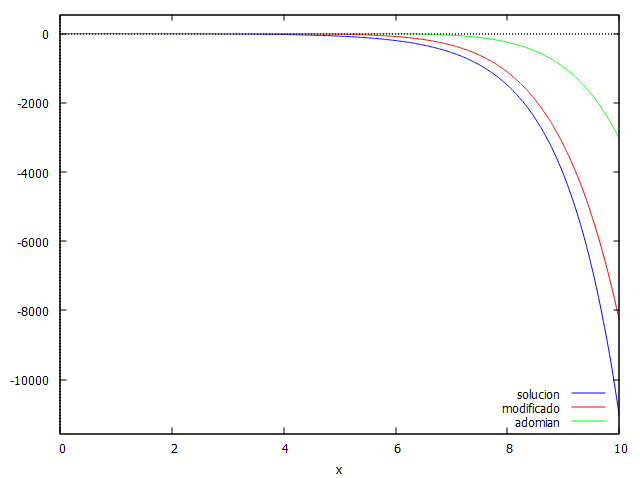
\includegraphics[width=0.8\textwidth]{ejemplo_adomian}
		\caption{Comparación de la solución para 5 iteraciones con el método de Adomian y el método modificado}
		\label{fig:adomian1}
	\end{figure}
	\begin{observacion}
		Podemos ver como efectivamente la convergencia en el método modificado es mucho más rápida que en el método de Adomian ya que con sólo 5 iteraciones ya se aproxima mucho mejor a la solución.
\end{observacion}
\end{ejemplo}

\subsection{Método de la solución en series}
\begin{definicion}
	Una función real $u(x)$ se llama \textit{analítica} si existe derivada de cualquier orden de forma que la serie de Taylor en cualquier punto $b$ de su dominio
	\begin{equation}
		u(x) = \sum_{k=0}^{\infty}\dfrac{f^{(k)}(b)}{k!}(x-b)^k,
	\end{equation}
	converge a $f(x)$ en un entorno de $b$.
\end{definicion}
Por simplicidad, escribiremos la forma genérica de la serie de Taylor en $x = 0$ como
\begin{equation}\label{eq:serie1}
	u(x) = \sum_{n=0}^{\infty}a_nx^n.
\end{equation}
\begin{observacion}
	Si $f$ es analítica en todo punto de un intervalo $I$, entonces, la propia definición nos garantiza que $f \in \mathcal{C}^\infty(I)$. Sin embargo, el recíproco no es cierto, como prueba el siguiente ejemplo bien conocido (véase en \cite{ejemploanalitica}):
	\begin{ejemplo}
		Sea la función
		\begin{equation}
			f(x) = \left\lbrace\begin{array}{c} e^{-1/x^2} \qquad x > 0 \\ 0 \qquad \qquad x \leqslant 0 \end{array}\right.
		\end{equation}
		Esta función es $\mathcal{C}^\infty(\R)$, ya que todas sus derivadas existen y son continuas en cualquier punto. Sin embargo, no es analítica en $x = 0$. La serie de Taylor alrededor de $x=0$ se reduce a una serie de potencias de ceros. Por lo tanto, no se puede representar como una serie de potencias convergente en un entorno de $x=0$.
	\end{ejemplo}
\end{observacion}
Vamos a presentar un método muy útil, que se basa principalmente en la serie de Taylor para funciones analíticas, y resolverá ecuaciones integrales de Volterra. Podemos apreciar que guarda cierta similitud con Adomian, ya que de igual forma expresamos $u$ como la suma de cierta serie.

Asumimos que la solución $u(x)$ de la ecuación integral de Volterra
\begin{equation}
	u(x) = f(x) + \int_0^x K(x,t)u(t)dt,
\end{equation}
es analítica, es decir, posee una solución en forma de serie de Taylor, donde los coeficientes $a_n$ se determinarán de forma recursiva. Sustituimos~\eqref{eq:serie1} en ambos miembros y obtenemos
\begin{equation}\label{eq:serie2}
	\sum_{n=0}^{\infty}a_nx^n = T(f(x)) + \int_{0}^{x}K(x,t)(\sum_{n=0}^{\infty}a_nt^n)dt,
\end{equation}
o por simplicidad usamos
\begin{equation}
	a_o + a_1x + a_2x^2 + \cdots = T(f(x)) + \int_{0}^{x}K(x,t) (a_0+a_1t+a_2t^2+\cdots)dt,
\end{equation}
donde $T(f(x))$ es la serie de Taylor para $f(x)$. La ecuación integral se convertirá en una integral tradicional donde en vez de integrar la función desconocida $u(x)$, se integrarán términos de la forma $t^n,n\geqslant0$. Al estar en búsqueda de una solución en series, si la función $f(x)$ incluye funciones elementales, deberemos incluir sus desarrollos en forma de Taylor.

Primero integramos la parte derecha de la integral en~\eqref{eq:serie2} y tomamos los coeficientes de las potencias de $x$. Después igualamos los coeficientes de ambos lados para obtener una relación de recurrencia con $a_j, j\geqslant0$. Resolver la recurrencia nos llevará a determinar completamente los coeficientes $a_j, j\geqslant0$.

Ahora la solución en series se sigue inmediatamente de sustituir estos coeficientes. La solución exacta se obtendrá si existe, y si no, la serie obtenida se podrá utilizar con objetivos numéricos. En este caso, a más términos evaluemos, mayor precisión obtendremos.

Veamos un ejemplo para dejar claro este método:
\begin{ejemplo}
	Vamos a resolver la ecuación integral de Volterra
	\begin{equation}
		u(x) = 1 - x \sin x + \int_{0}^{x} tu(t)dt.
	\end{equation}
	Sustituyendo la serie en ambos lados y utilizando la expansión en serie de Taylor para el seno obtenemos:
	\begin{equation}
		a_0 + a_1x + a_2x^2 + a_3x^3 + a_4x^4 +\cdots = 1 - x(x-\dfrac{x^3}{3!} + \cdots) + \int_{0}^{x}t(a_0+a_1t+a_2t^2+\cdots)dt.
	\end{equation}
	Integrando el lado derecho y quedándonos con los coeficientes encontramos
	\begin{equation}
		a_0 + a_1x + a_2x^2 + a_3x^3 + a_4x^4 + \cdots = 1+(\dfrac{1}{2}a_0-1)x^2+\dfrac{1}{3}a_1x^3+(\dfrac{1}{6}+\dfrac{1}{4}a_2)x^4+\cdots
	\end{equation}
	Igualando los coeficientes de las potencias de $x$,
	\begin{align}
		a_0&=1,          &  a_1&=0,      \\
		a_2&=\dfrac{1}{2}a_0-1,   &  a_3&=\dfrac{1}{3}a_1 = 0, \\
		a_4&=\dfrac{1}{6}+\dfrac{1}{4}a_2 = \dfrac{1}{4!},
	\end{align}
	y para $n\geqslant0$,
	\begin{equation}
		a_{2n+1} = 0, \qquad a_{2n} = \dfrac{(-1)^n}{(2n)!}, \qquad n \geqslant 0.
	\end{equation}
	La solución en forma de serie viene dada por
	\begin{equation}
		u(x) = 1 - \dfrac{1}{2!}x^2 + \dfrac{1}{4!}x^4-\dfrac{1}{6!}x^6+\cdots
	\end{equation}
	que nos da la solución exacta
	\begin{equation}
		u(x) = \cos x.
	\end{equation}
	En la \autoref{fig:sol_suma} mostramos la comparación de la suma parcial $v(x) = 1 - \dfrac{1}{2!}x^2 + \dfrac{1}{4!}x^4-\dfrac{1}{6!}x^6+\dfrac{1}{8!}x^8$ con la solución exacta $u(x)$, se aprecia que la aproximación es bastante buena.
	\begin{figure}[h!]
		\centering
		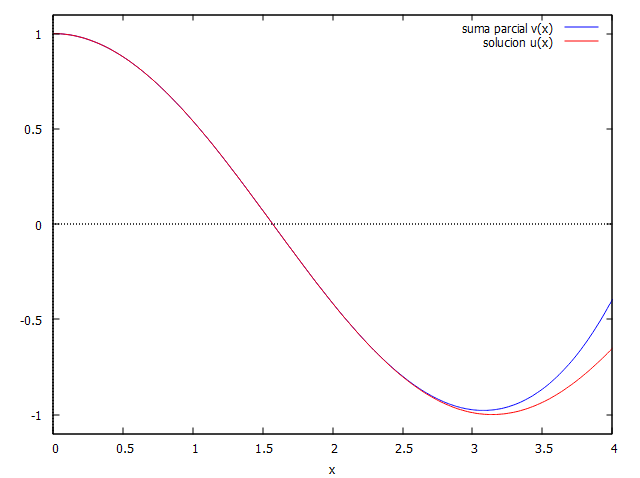
\includegraphics[width=0.8\textwidth]{suma_parcial_sol}
		\caption{Comparación de la solución exacta con la suma parcial $v(x)$}
		\label{fig:sol_suma}
	\end{figure}
\end{ejemplo}

\section{Métodos iterativos}

\subsection{Método de iteración variacional (VIM)}
Este método ha sido desarrollado por Ji-Huan He en sus libros \cite{VIM1} y \cite{VIM2}, y ha demostrado ser eficaz y seguro para estudios numéricos y analíticos. El método proporciona aproximaciones sucesivas que convergen rápidamente a la solución exacta en forma de serie, siempre que exista. Sin embargo, en el caso de que no se pueda obtener la solución exacta, la serie resultante se puede utilizar para fines numéricos. Asimismo, una de las ventajas que tiene este método es que puede abordar problemas tanto lineales como no lineales de la misma forma sin necesidad de añadir más restricciones. Lo vamos a incluir para ilustrar un método que es esencialmente no lineal, aunque no sea el objeto de estudio de esta memoria. Vamos a presentar los pasos principales del método:

Consideramos la ecuación diferencial:
\begin{equation}\label{eq:miv1}
	Lu + Nu = g(t),
\end{equation}
donde \textit{L y N} son operadores lineales y no lineales respectivamente , y $g(t)$ es el término no homogéneo.

El método de iteración variacional presenta un funcional de corrección para la ecuación~\eqref{eq:miv1} de la forma:
\begin{equation}\label{eq:miv2}
	u_{n+1}(x) = u_n(x) + \int_{0}^{x} \lambda(\xi)(Lu_n(\xi) + N\tilde{u}_n(\xi) - g(\xi))d\xi,
\end{equation}
donde $\lambda$ es un multiplicador de Lagrange general.
\begin{observacion}
	Nótese que en este método, $\lambda$ puede ser una constante o una función, y $\tilde{u}_n$ es un valor restringido, por tanto se comporta como una constante, luego $ \tilde{u}'_n = 0$.
\end{observacion}
Para un uso completo de este método, deberíamos seguir dos pasos:
\begin{enumerate}
	\item Determinar el multiplicador de Lagrange $\lambda(\xi)$ que será identificado de forma óptima.
	\item Una vez determinado $\lambda$, sustituimos el resultado en~\eqref{eq:miv2} donde se deberían omitir las restricciones.
\end{enumerate}
Derivando en~\eqref{eq:miv2} con respecto a la variable independiente $u_n$, obtenemos
\begin{equation}
	\dfrac{d u_{n+1}}{d u_n} = 1 + \dfrac{d}{d u_n}(\int_{0}^{x} \lambda(\xi)(Lu_n(\xi)+N\tilde{u}_n(\xi)-g(\xi))d\xi),
\end{equation}
o equivalentemente si multiplicamos por $du_n$:
\begin{equation}\label{eq:miv3}
	d u_{n+1} = d u_n + (\int_{0}^{x} \lambda (\xi)(Lu_n(\xi))d\xi).
\end{equation}
Para determinar el multiplicador de Lagrange $\lambda(\xi)$ normalmente se utiliza la integración por partes. Por ejemplo, si tenemos $Lu_n(\xi) = u'_n(\xi)$ en~\eqref{eq:miv3}, entonces se convierte en
\begin{equation}
	d u_{n+1} = d u_n +(\int_{0}^{x} \lambda (\xi)(u'_n(\xi))d\xi).
\end{equation}
Integrando por partes obtenemos
\begin{equation}
	d u_{n+1} = d u_n + \lambda(\xi)u_n(\xi) - \int_{0}^{x} \lambda'(\xi) d u_n(\xi)d\xi.
\end{equation}
o equivalentemente
\begin{equation}
	d u_{n+1} = d u_n(\xi)(1 + \lambda |_{\xi = x}) - \int_{0}^{x} \lambda'd u_nd\xi.
\end{equation}
La condición final de $u_{n+1}$ requiere que $d u_{n+1} = 0$. Esto significa que la parte izquierda vale cero, y por tanto la parte derecha también debería valer cero, lo que nos lleva a las condiciones:
\begin{equation}
	1 + \lambda |_{\xi = x} = 0, \qquad \lambda'|_{\xi = x} = 0.
\end{equation}
Lo que al final nos da
\begin{equation}
	\lambda = -1.
\end{equation}
Una vez hemos determinado el multiplicador de Lagrange $\lambda(\xi)$, las sucesivas aproximaciones $u_{n+1}, n \geqslant 0$, de la solución $u(x)$ se obtendrán fácilmente al usar la función selectiva $u_0(x)$. Sin embargo, para una rápida convergencia, la función $u_0(x)$ se debe seleccionar utilizando las primeras condiciones como siguen:
\begin{align}
	u_0(x) &= u(0),  \shorteqnote{para la primera derivada $u'_n$}  &   \\
	u_0(x) &= u(0) + xu'(0),  \shorteqnote{para la segunda derivada $u''_n$}  &   \\
	u_0(x) &= u(0) + xu'(0) + \dfrac{1}{2!}x^2u''(0), \qquad \qquad \qquad \shorteqnote{para la tercera derivada $u'''_n$}
\end{align}
y así sucesivamente. Por tanto, tenemos la solución 
\begin{equation}
	u(x) = \lim_{n\rightarrow \infty} u_n(x).
\end{equation}
Es decir, el funcional de corrección nos dará varias aproximaciones, y por tanto, la solución exacta se obtiene como el límite de todas estas sucesivas aproximaciones.

La determinación del multiplicador de Lagrange juega un papel muy importante para llegar a la solución del problema. A continuación, mostramos un esquema correspondiente al multiplicador de Lagrange y su funcional de corrección para un caso general de orden n:
	\begin{align}
	u^{(n)} + f(u(\xi),u'(\xi&),...,u^{(n)}(\xi)) = 0, \lambda = (-1)^n\dfrac{1}{(n-1)!}(\xi - x)^{(n-1)},      &   \\
	u_{n+1} = u_n + (-1)^n & \int_{0}^{x} \dfrac{1}{(n-1)!}(\xi - x)^{(n-1)}[u'''_n + f(u_n,...,u^{(n)}_n)]d\xi,    &
\end{align}
para todo $n \geqslant 1$.

Para utilizar el método de iteración variacional y resolver ecuaciones integrales de Volterra, es necesario convertir la ecuación integral a un problema de valores iniciales equivalente o a una ecuación integro-diferencial.

Vamos a examinar el problema de valores iniciales obtenido utilizando el método de iteración variacional como veremos en el siguiente ejemplo:
\begin{ejemplo}
	Resolveremos la siguiente ecuación integral de Volterra usando el método de iteración variacional:
	\begin{equation}
		u(x) = 1 + \int_{0}^{x}u(t)dt.
	\end{equation}
	Usando el Teorema Fundamental del Cálculo para derivar ambos lados de la ecuación, obtenemos
	\begin{equation}\label{eq:miv4}
		u'(x) - u(x) = 0.
	\end{equation}
	Sustituyendo $x = 0$, tenemos la condición inicial $u(0) = 1.$ Ahora, utilizando el método de iteración variacional, el funcional de corrección para la ecuación~\eqref{eq:miv4} es
	\begin{equation}\label{eq:miv5}
		u_{n+1}(x) = u_n(x) + \int_{0}^{x} \lambda (\xi) (u'_n(\xi) - \tilde{u}_n(\xi))d\xi.
	\end{equation}
	Usando la fórmula del esquema visto anteriormente para el caso $n = 1$ llegamos a que 
	\begin{equation}
		\lambda = -1.
	\end{equation}
	Sustituyendo el valor del multiplicador de Lagrange $\lambda = -1$ en el funcional nos da la fórmula iterativa:
	\begin{equation}
		u_{n+1}(x) = u_n(x) - \int_{0}^{x} (u'_n(\xi) - u_n(\xi))d\xi.
	\end{equation}
	Como dijimos anteriormente, podemos usar la condición inicial $u_0(x) = u(0) = 1.$ Usando esta selección en~\eqref{eq:miv5} obtenemos las siguientes aproximaciones sucesivas:
	\begin{align}
		u_0(x) &= 1,      &   \\
		u_1(x) &= 1 - \int_{0}^{x} (u'_0(\xi) - u_0(\xi))d\xi = 1 + x,    & \\
		u_2(x) &= 1 + x - \int_{0}^{x} (u'_1(\xi) - u_1(\xi))d\xi = 1 + x + \dfrac{1}{2!}x^2,    & \\
		u_3(x) &= 1 + x + \dfrac{1}{2!}x^2 - \int_{0}^{x} (u'_2(\xi) - u_2(\xi))d\xi = 1 + x + \dfrac{1}{2!}x^2 + \dfrac{1}{3!}x^3,    &
	\end{align}
	y así sucesivamente. El VIM admite el uso de 
	\begin{align}
		u(x) &= \lim_{n \rightarrow \infty} u_n(x),      &   \\
		&= \lim_{n \rightarrow \infty} (1 + x + \dfrac{1}{2!}x^2 + \dfrac{1}{3!}x^3 + ... + \dfrac{1}{n!}x^n)
	\end{align}
	con lo que obtenemos la solución exacta
	\begin{equation}
		u(x) = e^x.
	\end{equation}
	En la \autoref{fig:sol_vim} mostramos la comparación de la suma parcial $v(x) = 1 + \dfrac{1}{2!}x^2 + \dfrac{1}{3!}x^3+\dfrac{1}{4!}x^4$ con la solución exacta $u(x)$, se aprecia que la aproximación es bastante buena.
	\begin{figure}[h!]
		\centering
		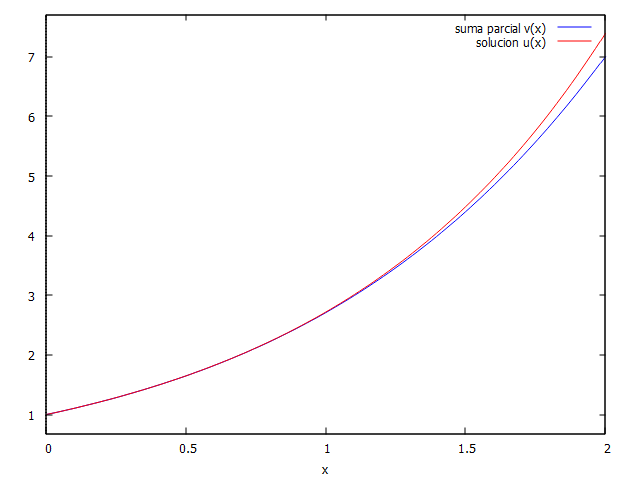
\includegraphics[width=0.8\textwidth]{grafica_vim}
		\caption{Comparación de la solución exacta con la suma parcial $v(x)$}
		\label{fig:sol_vim}
	\end{figure}
\end{ejemplo}

\subsection{Método de aproximaciones sucesivas}
El método de aproximaciones sucesivas, también conocido como el \textit{método de iteración de Picard}, nos proporciona un esquema que puede ser utilizado para resolver problemas de valores iniciales o ecuaciones integrales. Este método encuentra aproximaciones sucesivas que convergen a la solución a partir de una inicial, llamada la \textit{aproximación inicial}. Como veremos, la aproximación inicial puede ser cualquier función real que se utilizará en una relación recurrente para determinar las otras aproximaciones.

Dada la ecuación integral lineal de Volterra de segunda clase
\begin{equation}
	u(x) = f(x) +\int_{0}^{x} K(x,t)u(t)dt,
\end{equation}
donde $u(x)$ es la función desconocida a determinar, $K(x,t)$ es el núcleo, y $\lambda$ un parámetro. El método de las aproximaciones sucesivas introduce la siguiente relación de recurrencia
\begin{equation}\label{eq:wowo}
	u_n(x) = f(x) + \int_{0}^{x} K(x,t)u_{n-1}(t)dt, \qquad n \geqslant 1,
\end{equation}
donde la aproximación inicial $u_0(x)$ puede ser cualquier función real, a diferencia de Adomian. Siempre empezamos con una suposición inicial para $u_0(x)$, normalmente se suele elegir $0$ ó $f(x)$.

La convergencia de $u_n(x)$ está justificada con el estudio del capítulo $2$, teniendo en cuenta que 
\begin{equation}
	u = \sum_{j=0}^{\infty}L^jf,
\end{equation}
siendo $L$ el operador lineal visto en~\eqref{ref_operador}, que 
\begin{equation}
	u_n = \sum_{j=0}^{n}L^jf,
\end{equation}
y que el papel de $f$ ($=u_0$) lo puede jugar cualquier otra función continua $g$, ya que se tendría:
\begin{align}
		u_0 &= g \\ u_1 &= f+Lg \\ \vdots \\ u_n &= (\sum_{j=0}^{n-1}L^jf)+L^ng.
\end{align}
donde $L^ng \rightarrow 0$. Es más, en el mencionado capítulo $2$ obtuvimos cotas del error para este método.
En la siguiente observación vamos a ver algunas diferencias entre los métodos iterativos que hemos visto.
\begin{observacion}
	Es interesante ver que mientras que el método de iteración variacional utiliza la siguiente fórmula iterativa
	\begin{equation}
		u_{n+1}(x) = u_n(x) + \int_{0}^{x} \lambda(\xi)(\dfrac{\partial u_n(\xi)}{\partial \xi}-\tilde{u}_n(\xi))d\xi,
	\end{equation}
	el método de aproximaciones sucesivas utiliza la siguiente:
	\begin{equation}
		u_n(x) = f(x) + \int_{0}^{x} K(x,t)u_{n-1}(t)dt, \qquad n \geqslant 1,
	\end{equation}
\end{observacion}
Podemos resumir las diferencias entre ambas fórmulas de la siguiente forma:
\begin{enumerate}
	\item La primera fórmula contiene el multiplicador de Lagrange $\lambda$ que debería ser determinado antes de aplicar la fórmula. Sin embargo, la fórmula de aproximaciones sucesivas no requiere el uso de $\lambda$.
	\item La fórmula de iteración variacional permite el uso de la restricción $\tilde{u}_n(\xi)$ donde $\tilde{u}'_n(\xi) = 0.$ La segunda fórmula no requiere esta restricción.
	\item La primera fórmula se aplica a un ODE equivalente a la ecuación integral, mientras que la segunda fórmula se aplica directamente a la fórmula iterativa de la propia ecuación integral.
\end{enumerate}

Vamos a ilustrar este método con un ejemplo para que se vea más claro.
\begin{ejemplo}
	Vamos a resolver la siguiente ecuación integral de Volterra:
	\begin{equation}
		u(x) = 1 + x + \dfrac{1}{2}x^2 + \dfrac{1}{2}\int_{0}^{x}(x-t)^2u(t)dt.
	\end{equation}
	Para la aproximación inicial $u_0(x)$, seleccionamos
	\begin{equation}
		u_0(x) = 0.
	\end{equation}
	El método de las aproximaciones sucesivas nos permite el uso de la siguiente fórmula iterativa
	\begin{equation}
		u_{n+1}(x) = 1 + x + \dfrac{1}{2}x^2 + \dfrac{1}{2}\int_{0}^{x}(x-t)^2u_n(t)dt, \qquad n \geqslant 0.
	\end{equation}
	Sustituyendo la aproximación inicial obtenemos:
	\begin{align}
		u_1(x) &= 1 + x + \dfrac{1}{2}x^2 + \dfrac{1}{2}\int_{0}^{x}(x-t)^2u_0(t)dt = 1 + x + \dfrac{1}{2!}x^2,   & \\
		u_2(x) &= 1 + x + \dfrac{1}{2!}x^2 + \dfrac{1}{3!}x^3 + \dfrac{1}{4!}x^4, + \dfrac{1}{5!}x^5,   & \\
		u_3(x) &= 1 + x + \dfrac{1}{2!}x^2 + \dfrac{1}{3!}x^3 + \dfrac{1}{4!}x^4, + \dfrac{1}{5!}x^5 + \dfrac{1}{6!}x^6 + \dfrac{1}{7!}x^7 + \dfrac{1}{8!}x^8,     &
	\end{align}
	y así sucesivamente. La solución $u(x)$ viene dada por
	\begin{equation}
		u(x) = \lim_{n \rightarrow \infty} u_{n+1}(x) = e^x.
	\end{equation}
	La solución de este ejemplo es idéntica a la que podemos ver en la \autoref{fig:sol_vim} del método de iteración variacional.
\end{ejemplo}

\section{Otros métodos}

\subsection{Fenómeno de los términos de ruido}
Esta nueva técnica depende principalmente de los llamados \textit{términos de ruido}, y ha demostrado una rápida convergencia hacia la solución, se puede utilizar tanto para ecuaciones integrales como para ecuaciones diferenciales (véase \cite{WazWaz}).

Los términos con ruido, si existen entre las componentes $u_0(x)$ y $u_1(x)$, nos proporcionarán la solución exacta utilizando sólo las dos primeras iteraciones. Vamos a destacar los conceptos principales de estos términos:
\begin{enumerate}
	\item Los \textit{términos de ruido} se definen como los mismos términos con signos opuestos en las componentes $u_0(x)$ y $u_1(x)$. Pueden aparecer otros términos de ruido entre otras componentes, pero a nosotros nos interesarán los que aparezcan en las dos primeras.
	\item Al cancelar los términos de ruido entre $u_0(x)$ y $u_1(x)$, aunque $u_1(x)$ contenga términos adicionales, los términos restantes que no han sido cancelados de $u_0(x)$ podrían proporcionar la solución exacta de la ecuación integral. Sin embargo, esto no siempre va a ser así, la aparición de términos de ruido entre $u_0(x)$ y $u_1(x)$ no tiene por qué garantizar la obtención de la solución exacta. Por lo tanto, es necesario demostrar que los términos no cancelados de $u_0(x)$ satisfacen la ecuación integral dada. 
	
	Por otro lado, si los términos no cancelados de $u_0(x)$ no cumplieran con la ecuación integral dada, o los términos de ruido no aparecieran entre $u_0(x)$ y $u_1(x)$, entonces sería necesario determinar más componentes de $u(x)$ para obtener la solución en forma de serie.
	\item Los términos de ruido aparecen en tipos específicos de ecuaciones no homogéneas, sin embargo, no aparecen en ecuaciones homogéneas.
	\item Hay una condición necesaria para que se produzca la aparición de los términos de ruido, y es que la primera componente $u_0(x)$ debe contener la solución exacta $u(x)$, entre otros términos. Además, se demostró que la condición de no homogeneidad de la ecuación no siempre garantiza la aparición de los términos de ruido. Para más información acerca de los términos de ruido o la demostración de esta condición véase \cite{WazWaznoise}, \cite{WazWaz1} y \cite{WazWaz2}.
\end{enumerate}
Vamos a ilustrar la utilidad de los términos de ruido con un ejemplo:
\begin{ejemplo}
	Resolveremos la siguiente ecuación integral de Volterra:
	\begin{equation}
		u(x) = 8x + x^3 - \dfrac{3}{8} \int_{0}^{x} tu(t)dt.
	\end{equation}
	Establecemos la relación de recurrencia siguiendo el método estándar de Adomian:
	\begin{align}
		u_0(x) &= 8x + x^3,      &   \\
		u_1(x) &= - \dfrac{3}{8} \int_{0}^{x} tu(t)dt = - \dfrac{3}{40}x^5-x^3.    &
	\end{align}
	Podemos ver que $\pm x^3$ aparecen en $u_0(x)$ y $u_1(x)$, además con signos opuestos, por tanto es un término de ruido. Cancelando este término de la primera componente $u_0(x)$ obtenemos la solución exacta:
	\begin{equation}
		u(x) = 8x,
	\end{equation}
	que satisface la ecuación integral.
	\begin{observacion}
		Si hubiéramos elegido el método modificado, seleccionamos $u_0(x) = 8x$, luego tenemos que $u_1(x) = 0$. Por tanto, obtenemos el mismo resultado.
	\end{observacion}
\end{ejemplo}

\subsection{Método de la Transformada de Laplace}
Es una técnica muy potente que es capaz de resolver problemas de valores iniciales y ecuaciones integrales. Antes de aplicar el método, vamos a ver algunos conceptos importantes.

Si el núcleo $K(x,t)$ de la ecuación integral depende de la diferencia $x - t$, entonces se llama \textit{núcleo de diferencia}. Y podemos expresar la ecuación integral de la siguiente forma:
\begin{equation}\label{eq:lap1}
	u(x) = f(x) + \int_0^x K(x - t)u(t)dt.
\end{equation}
Considerando dos funciones $f_1(x)$ y $f_2(x)$ que poseen las condiciones necesarias para la existencia de la transformada de Laplace, sean las transformadas de Laplace para las funciones $f_1(x)$ y $f_2(x)$ dadas por:
\begin{equation}
	\mathcal{L}\{f_1(x)\} = F_1(s), \qquad \mathcal{L}\{f_2(x)\} = F_2(s).
\end{equation}
El \textit{producto de convolución de Laplace} de estas dos funciones se define como
\begin{equation}
	(f_1 \ast f_2)(x) = \int_{0}^{x} f_1(x-t)f_2(t)dt,
\end{equation}
ó
\begin{equation}
	(f_2 \ast f_1)(x) = \int_{0}^{x} f_2(x-t)f_1(t)dt,
\end{equation}
\begin{observacion}
	Recalcamos que
	\begin{equation}
		(f_1 \ast f_2)(x) = (f_2 \ast f_1)(x).
	\end{equation}
\end{observacion}
Podemos fácilmente ver que la transformada de Laplace del producto de convolución viene dada por:
\begin{equation}
	\mathcal{L}\{(f_1 \ast f_2)(x)\} = \mathcal{L}\{\int_{0}^{x}f_1(x-t)f_2(t)dt\} = F_1(s)F_2(s).
\end{equation}
Basándonos en este resumen de hechos bien conocidos, vamos a examinar ecuaciones integrales de Volterra específicas donde el núcleo es un núcleo de diferencia. Utilizaremos tanto la transformada de Laplace como su inversa.

Tomando la transformada de Laplace de ambos lados en~\eqref{eq:lap1} tenemos
\begin{equation}
	U(s) = F(s) + \mathcal{K}(s)U(s),
\end{equation}
donde
\begin{equation}
	U(s) = \mathcal{L}\{u(x)\}, \qquad \mathcal{K}(s) = \mathcal{L}\{K(x)\}, \qquad F(s) = \mathcal{L}\{f(x)\}.
\end{equation}
Resolviendo la ecuación para $U(s)$ obtenemos
\begin{equation}
	U(s) = \dfrac{F(s)}{1- \mathcal{K}(s)}, \qquad \mathcal{K}(s) \neq 1.
\end{equation}
La solución $u(x)$ se obtiene tomando la inversa de la transformada de Laplace en la ecuación anterior donde obtenemos:
\begin{equation}
	u(x) = \mathcal{L}^{-1}\{\dfrac{F(s)}{1- \mathcal{K}(s)}\}.
\end{equation}

\begin{ejemplo}
	Resolveremos la siguiente ecuación integral de Volterra utilizando el nuevo método:
	\begin{equation}
		u(x) = \sin x + \cos x + 2 \int_{0}^{x} \sin (x-t)u(t)dt.
	\end{equation}
	Vamos a aplicar la transformada de Laplace, y nos apoyaremos en su linealidad para obtener
	\begin{equation}
		\mathcal{L}\{u(x)\} = \mathcal{L}\{\sin x + \cos x\} + 2\mathcal{L}\{\sin (x-t) \ast u(x)\},
	\end{equation}
	y por tanto
	\begin{equation}
		U(s) = \dfrac{1}{s^2+1}+\dfrac{s}{s^2+1}+\dfrac{2}{s^2+1}U(s),
	\end{equation}
	o equivalentemente
	\begin{equation}
		U(s) = \dfrac{1}{s-1}.
	\end{equation}
	Tomando la inversa de Laplace en ambos lados obtenemos la solución exacta
	\begin{equation}
		u(x) = e^x.
	\end{equation}
\end{ejemplo}
\subsection{Métodos de cuadratura}
Son bien conocidos y de uso extendido. Nosotros hemos usado como referencia \cite{cuadratura} para desarrollarlos.

Sea $h > 0$ un tamaño fijo y sean $m, N$ tales que $Nh = B$, $m \leqslant N$. Entonces

\begin{equation}
	u(mh) - \int_{0}^{mh}K(mh,s)u(s)ds = f(mh), \qquad mh \in [0,B].
\end{equation}
Ahora, si usamos una fórmula de cuadratura de la forma $\displaystyle \int_{0}^{mh}F(s)ds = \displaystyle \sum_{j=0}^{m} w_{mj}F(jh),$ entonces la ecuación se aproxima por
\begin{equation}
	u(mh) - \sum_{j=0}^{m}w_{mj}K(mh,jh)u(jh) = f(mh),\qquad mh \in [0,B],
\end{equation}
donde $m = 1,2,...,N$ y tomando $x = 0$ tenemos el valor inicial $u(0) = f(0)$. Esto nos da el sistema de ecuaciones lineales (por tanto, resoluble sin problema, al menos para órdenes bajos)
\begin{equation}
	\begin{dcases}
		u(0) = f(0), \\ w_{10}K(h,0)u(0)+(1-w_{11}K(h,h))u(h) = f(h), \\ w_{20}K(2h,0)u(0)+w_{21}K(2h,h)u(h)+(1-w_{22}K(2h,2h))u(2h) = f(2h), \\ \vdots \\ \displaystyle \sum_{j=0}^{N-1}w_{Nj}K(Nh,jh)u(jh)+(1-w_{NN}K(Nh,Nh))u(Nh) = f(Nh). 
	\end{dcases}
\end{equation}
La precisión del resultado depende de la elección de $h$, la suavidad de $K(x,s)$ y $f(x)$, y la regla de cuadratura elegida. Por ejemplo, si elegimos la regla trapezoidal, el sistema se convierte en
\begin{equation}\label{eq:trapecio}
	\begin{dcases}
		u(mh) - h \displaystyle \sum_{j=0}^{m}``K(mh,jh)u(jh) = f(mh), \qquad m = 1,2,..., \\ u(0) = f(0),
	\end{dcases}
\end{equation}
que tiene un error de orden $O(h^2)$ cuando $h \rightarrow 0$.
\begin{ejemplo}
	Consideramos $K(x,s) = 12$, y tenemos
	\begin{equation}
		u(x) - \int_{0}^{x}12u(s)ds = f(x), \qquad x \in [0,B].
	\end{equation}
	Ahora, usando la regla de cuadratura del trapecio~\eqref{eq:trapecio} y escribimos la diferencia para $m = r$ y $m = r+1$ y restamos una de la otra, obteniendo la ecuación
	\begin{equation}
		(1-12h/2)u((r+1)h)-(1+12h/2)u(rh) = f((r+1)h)-f(rh) \equiv \Delta f(rh),
	\end{equation}
	para $r = 0,1,2,... .$ Luego la solución de la ecuación de Volterra viene dada por la recurrencia
	\begin{equation}
		u(rh) = \gamma^m f(0) + (1- 12h/2)^{-1}\sum_{s=0}^{m-1} \gamma^{m-s-1} s\Delta f(sh),
	\end{equation}
	\begin{figure}[h!]
		\centering
		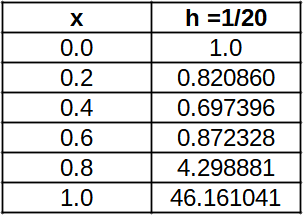
\includegraphics[width=0.35\textwidth]{tabla}
		\caption{Resultados del método para $h = 1/20$}
		\label{fig:tabla}
	\end{figure}
	donde $\gamma = (1 + 12h/2)/(1-12h/2)$. Tendremos que elegir $h$ de forma que $h \neq 2/12$. El error es de orden $O(h^2)$, se puede ver más detalladamente en \cite{cuadratura}.
	
	Vamos a tomar como ejemplo $f(x) = 13e^{-x}-12$, la solución exacta es $u(x) = e^{-x}$. Los resultados obtenidos con el método vienen dados en la \autoref{fig:tabla}.
\end{ejemplo}

Aunque no sea objeto de este trabajo, se pueden ver otros métodos interesantes para la resolución de las ecuaciones integrales de Fredholm de segunda clase, como métodos de proyección, el método de Nyström u otros métodos iterativos, para entrar más en detalle y profundizar un poco más, véase \cite{Atkinson} cap $12$.

\endinput
%------------------------------------------------------------------------------------
% FIN DEL CAPÍTULO. 
%------------------------------------------------------------------------------------


% !TeX root = ../libro.tex
% !TeX encoding = utf8
\chapter{Sistemas de ecuaciones integrales de Volterra de segunda clase}
\section{Introducción}
Los sistemas de ecuaciones integrales, lineales y no lineales, aparecen en muchas aplicaciones de ingeniería, física, química y modelos de crecimiento de poblaciones. Las ideas generales y las características esenciales de estos sistemas se pueden aplicar en muchos ámbitos.

Una gran variedad de métodos numéricos y analíticos se usan para manejar estos sistemas, pero la mayoría encuentran dificultades en términos del gran trabajo computacional, sobre todo cuando el sistema incluye varias ecuaciones integrales. Para evitar estas dificultades que normalmente se ven en los métodos tradicionales, vamos a utilizar algunos de los métodos introducidos en el capítulo anterior. El método de descomposición de Adomian y el método de la transformada de Laplace serán los que veremos.

Vamos a estudiar sistemas de ecuaciones integrales de Volterra de segunda clase dadas por
\begin{equation}
	u(x) = f_1(x) + \int_{0}^{x}(K_1(x,t)u(t) + \tilde{K}_1(x,t)v(t)+...),
\end{equation}
\begin{equation}
	v(x) = f_2(x) + \int_{0}^{x}(K_2(x,t)u(t) + \tilde{K}_2(x,t)v(t)+...).
\end{equation}
Las funciones desconocidas $u(x), v(x), .... ,$ que se determinarán, aparecen dentro y fuera de la integral. Los núcleos $K_i(x,t)$ y $\tilde{K}_i(x,t)$ y la función $f_i(x)$ son funciones reales dadas. A continuación veremos los métodos para resolver estos sistemas.
\section{Método de descomposición de Adomian}
Como ya vimos anteriormente, este método descompone cada solución en una suma infinita de componentes, donde cada componente se determina de forma recursiva. Este método puede utilizarse en su forma estándar o combinando los términos de ruido. Además, el método de descomposición modificado se utilizará donde sea apropiado. Veamos un ejemplo para resolver un sistema de ecuaciones integrales de Volterra utilizando este método.
\begin{ejemplo}
	Partimos del siguiente sistema:
	\begin{equation}
		u(x) = x - \dfrac{1}{6}x^4 + \int_{0}^{x}((x-t)^2u(t) + (x-t)v(t))dt,
	\end{equation}
	\begin{equation}
		v(x) = x^2 - \dfrac{1}{12}x^5 + \int_{0}^{x}((x-t)^3u(t) + (x-t)^2v(t))dt.
	\end{equation}
	El método nos sugiere que los términos lineales $u(x)$ y $v(x)$ se descompongan como una suma infinita de componentes
	\begin{equation}
		u(x) = \sum_{n=0}^{\infty}u_n(x), \qquad v(x) = \sum_{n=0}^{\infty}v_n(x),
	\end{equation}
	donde $u_n(x)$ y $v_n(x)$, $n \geqslant 0$ son las componentes de $u(x)$ y $v(x)$ que encontraremos de forma recursiva.
	
	Sustituyendo las series en el sistema obtenemos
	\begin{equation}
		\sum_{n=0}^{\infty}u_n(x) = x - \dfrac{1}{6}x^4 + \int_{0}^{x}((x-t)^2\sum_{n=0}^{\infty}u_n(t) + (x-t)\sum_{n=0}^{\infty}v_n(t))dt,
	\end{equation}
	\begin{equation}
		\sum_{n=0}^{\infty}v_n(x) = x^2 - \dfrac{1}{12}x^5 + \int_{0}^{x}((x-t)^3\sum_{n=0}^{\infty}u_n(t) + (x-t)^2\sum_{n=0}^{\infty}v_n(t))dt.
	\end{equation}
	
	Las primeras componentes $u_0(x)$ y $v_0(x)$ se definen como todos los términos que no están dentro de la integral, luego transformamos el sistema en un conjunto de relaciones recursivas dadas por
	\begin{align}
		u_0(x) &= x - \dfrac{1}{6}x^4,      &   \\
		u_{k+1}(x) &= \int_{0}^{x} ((x-t)^2u_k(t) + (x-t)v_k(t))dt, \qquad k \geqslant0 ,   &
	\end{align}
	y
	\begin{align}
		v_0(x) &= x^2 - \dfrac{1}{12}x^5,      &   \\
		v_{k+1}(x) &= \int_{0}^{x} ((x-t)^3u_k(t) + (x-t)^2v_k(t))dt, \qquad k \geqslant0 .   &
	\end{align}
	Si hacemos la primera iteración obtenemos
	\begin{equation}
		u_0(x) = x - \dfrac{1}{6}x^4, \qquad u_1(x) = \dfrac{1}{6}x^4 - \dfrac{1}{280}x^7,
	\end{equation}
	y
	\begin{equation}
		v_0(x) = x^2 - \dfrac{1}{12}x^5, \qquad v_1(x) = \dfrac{1}{12}x^5 - \dfrac{11}{10080}x^8.
	\end{equation}
	Es obvio que los términos de ruido $\pm \dfrac{1}{6}x^4$ aparecen entre $u_0(x)$ y $u_1(x)$. Además, los términos de ruido $\pm \dfrac{1}{12}x^5$ aparecen entre $v_0(x)$ y $v_1(x)$. Si cancelamos estos términos de ruido en $u_0(x)$ y $v_0(x)$, el resto de términos restantes nos dan la solución exacta
	\begin{equation}
		(u(x), v(x)) = (x,x^2).
	\end{equation}
\end{ejemplo}

\section{Método de la transformada de Laplace}
Puesto que ya hemos explicado este método en profundidad en el capítulo anterior, vamos a mostrar directamente un ejemplo en el que veremos cómo se aplica a un sistema de ecuaciones integrales de Volterra.
\begin{ejemplo}
	Sea
	\begin{equation}
		u(x) = 1 - x^2 + x^3 + \int_{0}^{x}((x-t)u(t) + (x-t)v(t))dt,
	\end{equation}
	\begin{equation}
		v(x) = 1 - x^3 - \dfrac{1}{10}x^5 + \int_{0}^{x}((x-t)u(t) - (x-t)v(t))dt.
	\end{equation}
	Es importante darse cuenta que ambos núcleos son iguales, es decir, $K_1(x-t) = K_2(x-t) = x-t$. Tomando la transformada de Laplace en ambos lados de cada ecuación obtenemos
	\begin{equation}
		U(s) = \mathcal{L}\{u(x)\} = \mathcal{L}\{1 - x^2 + x^3\} + \mathcal{L}\{(x-t)\ast u(x) + (x-t) \ast v(x)\},
	\end{equation}
	\begin{equation}
		V(s) = \mathcal{L}\{v(x)\} = \mathcal{L}\{1 - x^3 - \dfrac{1}{10}x^5\} + 	\mathcal{L}\{(x-t)\ast u(x) - (x-t) \ast v(x)\}.
	\end{equation}
	Esto al mismo tiempo nos da
	\begin{equation}
		U(s) = \dfrac{1}{s} - \dfrac{2}{s^3} + \dfrac{6}{s^4} + \dfrac{1}{s^2}U(s) + \dfrac{1}{s^2}V(s),
	\end{equation}
	\begin{equation}
		V(s) = \dfrac{1}{s} - \dfrac{6}{s^4} - \dfrac{12}{s^6} + \dfrac{1}{s^2}U(s) 	- \dfrac{1}{s^2}V(s),
	\end{equation}
	Reorganizando un poco el sistema obtenemos
	\begin{equation}
		(1-\dfrac{1}{s^2})U(s) - \dfrac{1}{s^2}V(s) = \dfrac{1}{s} - \dfrac{2}{s^3} + \dfrac{6}{s^4},
	\end{equation}
	\begin{equation}
		(1+\dfrac{1}{s^2})V(s) - \dfrac{1}{s^2}U(s) = \dfrac{1}{s} - \dfrac{6}{s^4}	- \dfrac{12}{s^6}.
	\end{equation}
	Resolviendo el sistema para $U(s)$ y $V(s)$ tenemos como resultado
	\begin{equation}
		U(s) = \dfrac{1}{s} + \dfrac{3!}{s^4},
	\end{equation}
	\begin{equation}
		V(s) = \dfrac{1}{s} - \dfrac{3!}{s^4}.
	\end{equation}
	Tomando la inversa de la transformada de Laplace en ambos lados de cada ecuación, la solución exacta viene dada por
	\begin{equation}
		(u(x),v(x)) = (1 + x^3, 1 - x^3).
	\end{equation}
\end{ejemplo}

\endinput
%------------------------------------------------------------------------------------
% FIN DEL CAPÍTULO. 
%------------------------------------------------------------------------------------

% !TeX root = ../libro.tex
% !TeX encoding = utf8
\chapter{Existencia y unicidad de solución de la ecuación lineal integral de Volterra de segunda clase}
\section{Teorema de la serie geométrica y sus variantes}
El siguiente resultado se usa muy a menudo en análisis numérico y matemática aplicada. También es la forma que tenemos para analizar si tienen solución los problemas que están $"$cerca$"$ a otros problemas que sabemos que tienen solución única.
\begin{teorema}
	(Teorema de la serie geométrica) Sea X un espacio de Banach, $L \in \mathcal{L}(X)$. Suponemos
	\begin{equation}
		\lVert L \rVert \leq 1.
	\end{equation}
	Entonces $I - L$ es una biyección en X, su inversa es un operador lineal continuo,
	\begin{equation}
		(I-L)^{-1} = \sum_{n=0}^{\infty}L^n,
	\end{equation}
	y
	\begin{equation}\label{eq:teo1}
		\lVert (I-L)^{-1} \rVert \leqslant \dfrac{1}{1 - \lVert L \rVert}.
	\end{equation}
\end{teorema}
\begin{proof}
	Definimos una sucesión en $\mathcal{L}(X): M_n = \sum_{i=0}^{n}L^i, n \geqslant 0$. Para $p \geqslant 1$, 
	\begin{equation}
		\lVert M_{n+p} - M_n \rVert = \lVert \sum_{i=n+1}^{n+p}L^i \rVert \leqslant \sum_{i=n+1}^{n+p} \lVert L^i \rVert \leqslant \sum_{i=n+1}^{n+p} \lVert L \rVert^i.
	\end{equation}
	Usando que $\lVert L \rVert \leq 1$, tenemos
	\begin{equation}
		 \lVert M_{n+p} - M_n \rVert \leqslant \dfrac{\lVert L \rVert^{n+1}}{1 - \lVert L \rVert}.
	\end{equation}
	Por tanto,
	\begin{equation}
		\sup_{p \geqslant 1} \lVert M_{n+p} - M_n \rVert \rightarrow 0, \qquad n \rightarrow \infty,
	\end{equation}
	y \{$M_n$\} es una sucesión de Cauchy en $\mathcal{L}(X)$. Como $\mathcal{L}(X)$ es completo, hay un $M \in \mathcal{L}(X)$ tal que
	\begin{equation}
		\lVert M_{n} - M \rVert \rightarrow 0, \qquad n \rightarrow \infty.
	\end{equation}
	Usando la definición de $M_n$ y una simple manipulación algebraica,
	\begin{equation}
		(I-L)M_n = M_n(I-L) = I - L^{n+1}.
	\end{equation}
	Si $n \rightarrow \infty$ obtenemos
	\begin{equation}
		(I-L)M = M(I-L) = I.
	\end{equation}
	Esta relación implica que $(I-L)$ es una biyección, y
	\begin{equation}
		M = (I-L)^{-1} = \lim_{n \rightarrow \infty}\sum_{i=0}^{n}L^i = \sum_{n=0}^{\infty}L^n.
	\end{equation}
	Para probar la desigualdad~\eqref{eq:teo1}, observemos que
	\begin{equation}
		\lVert M_{n} \rVert \leqslant \sum_{i=0}^{n}\lVert L \rVert^i \leqslant \dfrac{1}{1 - \lVert L \rVert}.
	\end{equation}
	Tomando el límite en $n \rightarrow \infty$, obtenemos~\eqref{eq:teo1}.
\end{proof}
\begin{observacion}
	El teorema dice que bajo las hipótesis que hemos marcado, para cualquier $f \in X$, la ecuación
	\begin{equation}\label{eq:teo2}
		(I-L)u = f
	\end{equation}
	tiene solución única $u = (I-L)^{-1}f \in X$. Además, la solución depende continuamente de la parte derecha $f$: Siendo $(I-L)u_1 = f_1$ y $(I-L)u_2 = f_2$, de esto se sigue que
	\begin{equation}
		u_1 - u_2 = (I-L)^{-1}(f_1 - f_2),
	\end{equation}
	y por tanto,
	\begin{equation}
		\lVert u_1 - u_2 \rVert \leqslant c \lVert f_1 - f_2 \rVert
	\end{equation}
	con $c = 1/(1 - \lVert L \rVert)$.
\end{observacion}
\begin{observacion}
	Este teorema también nos da una forma de aproximar la solución de la ecuación~\eqref{eq:teo2}. Bajo las hipótesis del teorema, tenemos
	\begin{equation}
		u = \lim_{n \rightarrow \infty}u_n
	\end{equation}
	donde
	\begin{equation}
		u_n = \sum_{j=0}^{n}L^jf.
	\end{equation}
\end{observacion}
Veamos a continuación un ejemplo en el que, gracias al teorema de la serie geométrica, veremos que una ecuación lineal integral tiene solución única.
\begin{ejemplo}\label{ej:1}
	Sea la siguiente ecuación:
	\begin{equation}
		\lambda u(x) - \int_{a}^{b}k(x,t)u(t)dy = f(x), \qquad a \leqslant x \leqslant b
	\end{equation}
	con $\lambda \neq 0$, $k(x,y)$ continua para $x,y \in [a,b]$, y $f \in \mathcal{C}[a,b]$. Sea $X = \mathcal{C}[a,b]$ con la norma $\lVert \cdot \rVert_\infty$. Simbólicamente, escribimos la ecuación como
	\begin{equation}
		(\lambda I-K)u = f,
	\end{equation}
	donde $K$ es un operador integral lineal gerenado por el núcleo $k(\cdot , \cdot )$. Nosotros también lo escribiremos a menudo como $(\lambda - K)u = f$, para aclarar la notación.
	
	Escribimos la ecuación de esta manera puesto que así se puede convertir en la forma que necesitamos para aplicar el teorema de la serie geométrica:
	\begin{equation}
		(I-L)u = \dfrac{1}{\lambda}f, \qquad L = \dfrac{1}{\lambda}K.
	\end{equation}
	Aplicando el teorema de la serie geométrica, afirmamos que si
	\begin{equation}
		\lVert L \rVert = \dfrac{1}{|\lambda |}\lVert K \rVert \leq 1,
	\end{equation}
	entonces $(I-L)^{-1}$ existe y
	\begin{equation}
		\lVert(I-L)^{-1}\rVert \leqslant \dfrac{1}{1 - \lVert L \rVert}.
	\end{equation}
	Equivalentemente, si
	\begin{equation}
		\lVert K \rVert = \max_{a\leqslant x\leqslant b}\int_{a}^{b}|K(x,t)|dt \leq |\lambda|,
	\end{equation}
	entonces $(\lambda I - K)^{-1}$ existe y 
	\begin{equation}
		\lVert (\lambda I - K)^{-1}\rVert \leqslant \dfrac{1}{|\lambda| - \lVert K \rVert }.
	\end{equation}
	Luego, para cualquier $f \in \mathcal{C}[a,b]$, la ecuación integral tiene solución única $u \in \mathcal{C}[a,b]$ y 
	\begin{equation}
		\lVert u \rVert_\infty \leqslant \lVert (\lambda I - K)^{-1} \rVert \lVert f \rVert_\infty \leqslant \dfrac{\lVert f \rVert_\infty}{|\lambda| - \lVert K \rVert }.
	\end{equation}
\end{ejemplo}
\begin{observacion}
	Gracias a la demostración del teorema podemos ver que para un operador lineal $L \in \mathcal{L}(X)$ sobre un espacio de Banach $V$, si $\lVert L \rVert \leq 1$, entonces la serie $\sum_{n=0}^{\infty}L^n$ converge en $\mathcal{L}(X)$ y el valor de la serie es el operador $(I-L)^{-1}$.
\end{observacion}
\subsection{Generalización del teorema}
Para motivar la generalización del teorema, vamos a considerar la ecuación integral de Volterra de segunda clase
\begin{equation}
	u(x) - \int_{0}^{x} K(x,t)u(t)dt = f(x), \qquad x \in [0,B],
\end{equation}
donde $B \geq 0$ y suponemos que el núcleo $K(x,t)$ es continuo para $0 \leqslant t \leqslant x \leqslant B$, y $f \in \mathcal{C}[0,B]$. Si aplicamos el teorema, tendremos que suponer una condición para poder concluir la existencia de solución única, de forma que
\begin{equation}
	\max_{x\in [0,B]}\int_{0}^{x} |K(x,t)|dt \leq 1.
\end{equation}
Sin embargo, podemos usar una variante del teorema de la serie geométrica sin importar el tamaño del núcleo $K(x,t)$, y garantizando la existencia de solución única. Simbólicamente, escribimos la ecuación integral como $(I-L)u = f$.
\begin{corolario}
	Sea X un espacio de Banach, $L \in \mathcal{L}(X)$. Suponemos que para algún entero $m \geqslant 1$ se cumple
	\begin{equation}
		\lVert L^m \rVert \leq 1.
	\end{equation}
	Entonces $I - L$ es una biyección en $X$, su inversa es un operador lineal acotado, y 
	\begin{equation}\label{eq:teo3}
		\lVert (I-L)^{-1} \rVert \leqslant \dfrac{1}{1 - \lVert L^m \rVert} \sum_{i=0}^{m - 1}\lVert L^i \rVert.
	\end{equation}
\end{corolario}
\begin{proof}
	Gracias al teorema de la serie geométrica, sabemos que $(I-L^m)^{-1}$ existe como un operador biyectivo acotado de $X$ en sí mismo,
	\begin{equation}
		(I - L^m)^{-1} = \sum_{j=0}^{\infty}L^{mj} 
	\end{equation}
	en $\mathcal{L}(X)$, y
	\begin{equation}
		\lVert (I - L^m)^{-1} \rVert \leqslant \dfrac{1}{1 - \lVert L^m \rVert}.
	\end{equation}
	De las igualdades
	\begin{equation}
		(I - L)(\sum_{i=0}^{m - 1}L^i) = (\sum_{i=0}^{m - 1}L^i)(I-L) = I - L^m,
	\end{equation}
	concluimos que $(I-L)$ es una biyección,
	\begin{equation}
		(I-L)^{-1} = (\sum_{i=0}^{m-1}L^i)(I-L^m)^{-1}
	\end{equation}
	y la desigualdad~\eqref{eq:teo3} se mantiene.
\end{proof}
\subsection{Un resultado de perturbación}
La \textit{perturbación} es una técnica en matemática aplicada que estudia una ecuación relacionándola con otra ecuación ``cercana'' para la cual existe un resultado que nos proporciona una solución. El siguiente teorema es una de las herramientas más utilizadas.

\begin{teorema}
	Sea $X$ y $Y$ espacios normados, siendo al menos uno de ellos completo. Suponemos que $L \in \mathcal{L}(X,Y)$ tiene inversa acotada $L^{-1}: Y \rightarrow X.$ Suponemos $M \in \mathcal{L}(X,Y)$ satisface
	\begin{equation}\label{eq:teo7}
		\lVert M-L \rVert < \dfrac{1}{\lVert L^{-1} \rVert}.
	\end{equation}
	Entonces $M:X\rightarrow Y$ es una biyección, $M^{-1} \in \mathcal{L}(Y,X)$ y 
	\begin{equation}\label{eq:teo5}
		\lVert M^{-1} \rVert \leqslant \dfrac{\lVert L^{-1} \rVert}{1 - \lVert L^{-1} \rVert \lVert L-M \rVert}.
	\end{equation}
	Además,
	\begin{equation}\label{eq:teo4}
		\lVert L^{-1} - M^{-1} \rVert \leqslant \dfrac{\lVert L^{-1} \rVert^2 \lVert L-M \rVert}{1 - \lVert L^{-1} \rVert \lVert L-M \rVert}.
	\end{equation}
	Para soluciones de las ecuaciones $Lx_1 = y$ y $Mx_2 = y,$ tenemos la acotación
	\begin{equation}\label{eq:teo6}
		\lVert x_1 - x_2 \rVert \leqslant \lVert M^{-1} \rVert \lVert (L-M)x_1 \rVert.
	\end{equation}
\end{teorema}
\begin{proof}
	Escribimos $M$ como una perturbación de $L$. Si $Y$ es completo, escribimos
	\begin{equation}
		M = [I - (L - M)L^{-1}]L;
	\end{equation}
	mientras que si $X$ es completo, escribiremos
	\begin{equation}
		M = L[I - L^{-1}(L - M)].
	\end{equation}
	Vamos a hacer la demostración en el caso de que $Y$ sea completo.
	El operador $(L-M)L^{-1} \in \mathcal{L}(Y)$ satisface
	\begin{equation}
		\lVert (L - M)L^{-1} \rVert \leqslant \lVert L - M \rVert \lVert L^{-1 \rVert} < 1.
	\end{equation}
	Luego por el teorema de la serie geométrica, $[I-(L-M)L^{-1}]^{-1}$ existe y además,
	\begin{equation}
		\lVert [I-(L-M)L^{-1}]^{-1} \rVert \leqslant \dfrac{1}{1 - \lVert (L-M)L^{-1}\rVert} \leqslant \dfrac{1}{1 - \lVert L^{-1} \rVert \lVert L-M \rVert }.
	\end{equation}
	$M^{-1}$ existe con
	\begin{equation}
		M^{-1} = L^{-1}[I-(L-M)L^{-1}]^{-1}
	\end{equation}
	y
	\begin{equation}
		\lVert M^{-1} \rVert \leqslant \lVert L^{-1} \rVert \lVert [I-(L-M)L^{-1}]^{-1} \rVert \leqslant \dfrac{\lVert L^{-1} \rVert}{1 - \lVert L^{-1} \rVert \lVert L-M \rVert}.
	\end{equation}
	Para probar~\eqref{eq:teo4}, escribimos
	\begin{equation}
		L^{-1} - M^{-1} = M^{-1}(M-L)L^{-1},
	\end{equation}
	tomando normas y usando~\eqref{eq:teo5}.
	
	Para~\eqref{eq:teo6},
	\begin{equation}
		x_1 - x_2 = (L^{-1} - M^{-1})y = M^{-1}(M-L)L^{-1}y = M^{-1}(M-L)x_1
	\end{equation}
	y aplicamos normas y acotaciones.
\end{proof}
Podemos resumir el teorema anterior en una frase: \textit{Un operador cercano a otro operador con inversa acotada, también tendrá inversa acotada.} Este es el marco de trabajo para innumerables resultados de existencia de soluciones para ecuaciones integrales y diferenciales.

\textbf{Pensar: consistencia, estabilidad y convergencia.}

\begin{ejemplo}
	Vamos a examinar si la ecuación integral tiene solución
	\begin{equation}\label{eq:ej1}
		\lambda u(x) - \int_{0}^{1}\sin(xt)u(t)dt = f(x), \qquad 0 \leqslant x \leqslant 1
	\end{equation}
	con $\lambda \neq 0$. De la discusión del ejemplo~\eqref{ej:1}, si
	\begin{equation}\label{ej:2}
		|\lambda| > \lVert K \rVert = \int_{0}^{1}\sin(t)dt = 1 - \cos(1) \approx 0.4597,
	\end{equation}
	entonces para cada $f \in \mathcal{C}[0,1]$, la ecuación admite una solución única $u \in \mathcal{C}[0,1]$.
	
	Para obtener más valores de $\lambda$ para los cuales nuestra ecuación tiene solución única, aplicamos el teorema de perturbación. Ya que $\sin(xt) \approx xt$ para valores pequeños de $|xt|$, comparamos la ecuación con
	\begin{equation}\label{eq:ej2}
		\lambda v(x) - \int_{0}^{1} xtv(t)dt = f(x), \qquad 0 \leqslant x \leqslant 1.
	\end{equation}
	Siguiendo la notación el teorema de perturbación, la ecuación~\eqref{eq:ej1} sería $Mu = f$, y~\eqref{eq:ej2} sería $Lv = f$. El espacio normado es $V = \mathcal{C}[0,1]$ con la norma $\lVert \cdot \rVert_\infty$, y $L,M \in \mathcal{L}(V)$.
	
	Podemos resolver la ecuación integral~\eqref{eq:ej2} de forma explícita. Suponiendo $\lambda \neq 0$, tenemos que cada solución $v$ toma la forma
	\begin{equation}
		v(x) = \dfrac{1}{\lambda}[f(x)+cx]
	\end{equation}
	para alguna constante $c$. Sustituyéndolo en la ecuación nos lleva a una fórmula para $c$, y entonces
	\begin{equation}
		v(x) = \dfrac{1}{\lambda}[f(x) + \dfrac{1}{\lambda - 1/3}\int_{0}^{1}xtf(t)dt], \qquad \lambda \neq 0,\dfrac{1}{3}.
	\end{equation}
	Esta relación define $L^{-1}f$ para toda $f \in \mathcal{C}[0,1]$.
	
	Para usar el teorema de perturbación, necesitamos medir algunas cantidades. Se puede calcular que
	\begin{equation}
		\lVert L^{-1} \rVert \leqslant \dfrac{1}{|\lambda|}(1 + \dfrac{1}{2|\lambda - 1/3|})
	\end{equation}
	y
	\begin{equation}
		\lVert L-M \rVert = \int_{0}^{1} (t - \sin t)dt = \cos(1) - \dfrac{1}{2} \approx 0.0403.
	\end{equation}
	La condición~\eqref{eq:teo7} viene de
	\begin{equation}\label{ej:3}
		\dfrac{1}{|\lambda|}(1+\dfrac{1}{2|\lambda - 1/3|}) < \dfrac{1}{\cos(1)-1/2}.
	\end{equation}
	En la \autoref{fig:4.1} podemos ver un gráfico de la parte izquierda de esta desigualdad. Si $\lambda$ es un número real, entonces hay tres casos a considerar: $\lambda > 1/3$, $0 < \lambda < 1/3$, y $\lambda < 0$. Para el caso $\lambda < 0$, la desigualdad es cierta si y sólo si $\lambda < \lambda_0 \approx -0.0881$, que es la raíz negativa de la ecuación
	\begin{equation}
		\lambda^2 - (\dfrac{5}{6} - \cos(1)) \lambda - \dfrac{5}{6}(\cos(1) - \dfrac{1}{2}) = 0.
	\end{equation} 
	Como consecuencia el teorema de perturbación, tenemos que si $\lambda < \lambda_0$, entonces nuestra ecuación integral tiene solución única para cualquier $f \in \mathcal{C}[0,1]$. Esto es una mejora significativa en comparación con el punto de partida que teníamos~\eqref{ej:2}.
\end{ejemplo}
\begin{figure}[htb!]
	\centering
	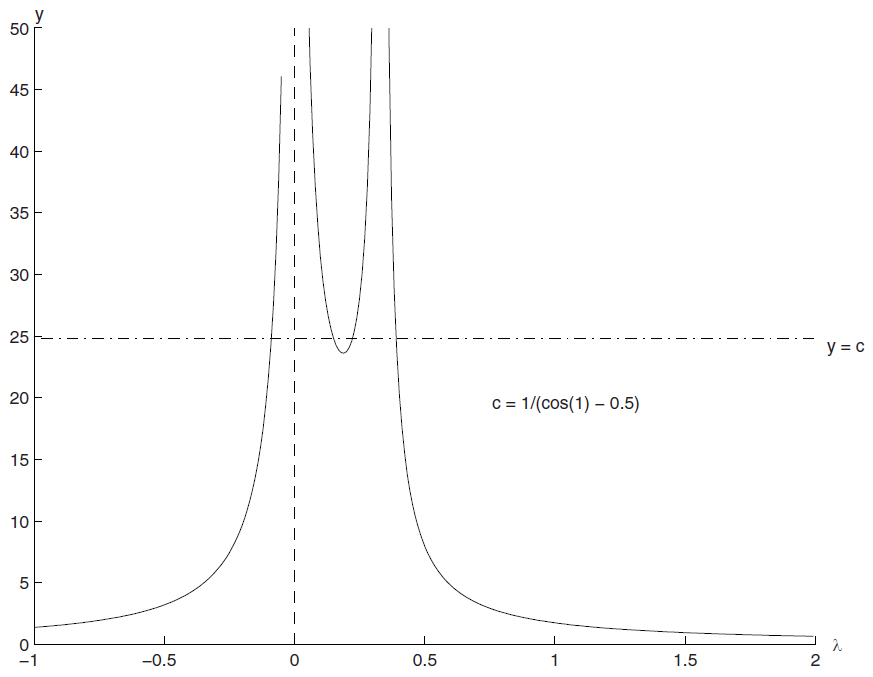
\includegraphics[width=\textwidth]{fig4.1}
	\caption{Gráfico de la parte izquierda de la desigualdad~\eqref{ej:3}}
	\label{fig:4.1}
\end{figure}

\endinput
%------------------------------------------------------------------------------------
% FIN DEL CAPÍTULO. 
%------------------------------------------------------------------------------------

% !TeX root = ../libro.tex
% !TeX encoding = utf8
\chapter{Equivalencia entre ecuaciones diferenciales y ecuaciones de Volterra}
A continuación veremos la equivalencia que existe entre ambos tipos de ecuaciones, más concretamente, veremos las ecuaciones diferenciales lineales como un caso particular de las ecuaciones de Volterra. Primero vamos a ver el caso escalar, y después lo haremos vectorialmente.
\section{Escalar}
Consideramos el PVI:
\begin{equation}
	x \in \mathcal{C}^1(0,B):\left\lbrace\begin{array}{c} x'(t) = a(t)x(t)+b(t) \\ x(0) = x_0 \end{array}\right.,\qquad t \in (0,B)
\end{equation}
La solución del PVI es de la forma
\begin{equation}
	x \in \mathcal{C}[0,B]: x = T(x)
\end{equation}
donde definimos el operador lineal $T$ como
\begin{equation}
	T: \mathcal{C}[0,B] \longrightarrow \mathcal{C}[0,B]
\end{equation}
\begin{equation}
	\qquad \qquad x \longmapsto T(x): [0,B] \rightarrow \R
\end{equation}
\begin{equation}
	\qquad \qquad \qquad \qquad \qquad \qquad \qquad \qquad (T(x))(t) = x_0 + \int_0^t(a(s)x(s)+b(s))ds
\end{equation}
Por tanto, vemos que la solución del PVI es un caso particular de la ecuación integral lineal de Volterra de segunda clase:
\begin{equation}
	x(t) = f(t) + \lambda \int_0^t K(t,s)x(s)ds,
\end{equation}
donde
\begin{equation}
	f(t) = x_0 + \int_0^t b(s)ds, \qquad K(t,s) = a(s), \qquad \lambda = 1.
\end{equation}
Para ver la equivalencia, aplicamos el Teorema Fundamental del Cálculo a la siguiente ecuación integral:
\begin{equation}
	x(t) = x_0 + \int_0^t (a(s)x(s)+b(s))ds,
\end{equation}
y obtenemos
\begin{equation}
	\left\lbrace\begin{array}{c} x'(t) = a(t)x(t)+b(t) \\ x(0) = x_0 \end{array}\right.,\qquad t \in (0,B).
\end{equation}
En definitiva, la solución del PVI inicial coincide con la solución de la ecuación de Volterra lineal de segunda clase.
\section{Vectorial}
INDICACIÓN:
En este caso, el PVI sería (y lo pongo entero), luego lo escribo de forma matricial y vectorial con las negritas. Después hago la misma equivalencia que en el caso escalar. Luego la conclusión entiendo que es la misma de forma vectorial? DUDA
\endinput
%------------------------------------------------------------------------------------
% FIN DEL CAPÍTULO. 
%----------------------------------------------------------------------------------
-

% !TeX root = ../libro.tex
% !TeX encoding = utf8
\chapter{Aplicación: Calentamiento y enfriamiento de edificios}
Como aplicación sobre lo estudiado anteriormente, vamos a formular un modelo matemático que describa la temperatura dentro de un edificio, como función de la temperatura exterior, el calor generado dentro del edificio y el calefactor o el aire acondicionado.

Un enfoque natural para modelar la temperatura dentro de un edificio es el uso del análisis por compartimentos.
\section{Edificio como habitación única}
Sea $T(t)$ la temperatura dentro del edificio en el instante $t$ y veamos al edificio como un único compartimento, es decir, sin estar dividido en varias habitaciones. Entonces la razón de cambio en la temperatura queda determinada por todos los factores que generan o disipan calor. Tomaremos en cuenta tres factores principales que afectan la temperatura dentro del edificio:
\begin{itemize}
	\item En primer lugar está el calor generado por las personas, las luces y las máquinas dentro del edificio. Esto causa una razón de incremento en la temperatura que denotaremos por $H(t)$.
	\item En segundo lugar está el calentamiento (o enfriamiento) proporcionado por la calefacción (o el aire acondicionado).  Esta razón de incremento (o decremento) en temperatura será representada por $U(t)$.
	\item El tercer factor es el efecto de la temperatura exterior $M(t)$ sobre la temperatura dentro del edificio. La evidencia experimental ha mostrado que este factor se puede modelar mediante la \textbf{ley de enfriamiento de Newton}.
	
	Esta ley establece que hay una razón de cambio de la temperatura $T(t)$ que es proporcional a la diferencia entre la temperatura exterior $M(t)$ y la temperatura interior $T(t)$. Es decir, la razón de cambio en temperatura del edificio debida a $M(t)$ es 
	\begin{equation}
		K[M(t) - T(t)].
	\end{equation}
	La constante positiva $K$ depende de las propiedades físicas del edificio, como la cantidad de puertas y ventanas o el tipo de aislamiento, pero $K$ no depende de $M$, $T$ o $t$. Por lo tanto, cuando la temperatura exterior es mayor que la temperatura interior, $M(t) - T(t) > 0$ y hay un incremento en la temperatura del edificio debido a $M(t)$. 
	
	Por otro lado, cuando la temperatura exterior es menor que la temperatura interior, entonces $M(t) - T(t) < 0$ y la temperatura del edificio disminuye.
\end{itemize}
En general, la razón de calentamiento adicional $H(t)$ y la razón de calefacción
(o enfriamiento) $U(t)$ quedan descritas en términos de energía por unidad de tiempo
(como las unidades térmicas británicas por hora). Sin embargo, al multiplicar por la
capacidad calórica del edificio (en unidades de cambio de temperatura por unidad de energía calórica), podemos expresar las dos cantidades $H(t)$ y $U(t)$ en términos de temperatura por unidad de tiempo.

En definitiva, vemos que 
\begin{equation}
	\dfrac{\partial T}{\partial t} = K[M(t) - T(t)] + H(t) + U(t),
\end{equation}
cuando la razón de calentamiento adicional $H(t)$ es siempre no negativa y $U(t)$ es positiva para la calefacción y negativa para el aire acondicionado. Como la ecuación es lineal, la resolveremos fácilmente escribiéndola en la forma canónica
\begin{equation}
	\dfrac{\partial T}{\partial t}(t) + P(t)T(t) = Q(t),
\end{equation}
donde
\begin{equation}
	P(t) := K,
\end{equation}
\begin{equation}\label{eq:apli1}
	Q(t) := KM(t) + H(t) + U(t),
\end{equation}
vemos que el factor integrante es
\begin{equation}
	\mu (t) = \exp(\int Kdt) = e^{Kt}.
\end{equation}
Para resolver la ecuación, multiplicamos $e^{Kt}$ e integramos:
\begin{equation}
	e^{Kt}\dfrac{\partial T}{\partial t}(t) + Ke^{Kt}T(t) = e^{Kt}Q(t),
\end{equation}
\begin{equation}
	e^{Kt}T(t) = \int e^{Kt}Q(t)dt + C.
\end{equation}
Al despejar $T(t)$ se tiene
\begin{equation}\label{eq:apli2}
	T(t) = e^{-Kt}\int e^{Kt}Q(t)dt + Ce^{-Kt}
\end{equation}
\begin{equation}
	= e^{-Kt}\{\int e^{Kt}[KM(t) + H(t) + U(t)]dt + C\}.
\end{equation}
A continuación vamos a resolver unos ejercicios sobre calentamiento y enfriamiento de edificios en el que tenemos solamente una habitación. Vamos a ver primero un ejemplo sencillo en el que suponemos la temperatura exterior constante:
\begin{ejemplo}
	Suponemos que al final del día (en el instante $t_0$), cuando las personas salen del edificio, la temperatura exterior permanece constante e igual a $M_0$, la razón de calentamiento adicional $H$ dentro del edificio se anula y la razón de uso del calefactor o el aire acondicionado $U$ también se anula. Determinar $T(t)$, dada la condición inicial $T(t_0) = T_0$.\\
	\textbf{Solución.} Con $M = M_0$, $H = 0$ y $U = 0$, la ecuación~\eqref{eq:apli2} se convierte en
	\begin{equation}
		T(t) = e^{-Kt}\{\int e^{Kt}KM_0dt+C\} = e^{-Kt}[M_0e^{Kt}+C] = M_0 + Ce^{-Kt}.
	\end{equation}
	Al hacer $t = t_0$ y usar el valor inicial $T_0$ de la temperatura, vemos que la constante $C$ es $(T_0 - M_0)e^{Kt_0}$. Por lo tanto,
	\begin{equation}
		T(t) = M_0 + (T_0 - M_0)e^{-K(t-t_0)}.
	\end{equation}
	Cuando $M_0 < T_0$, es decir, la temperatura exterior es menor que la interior, la solución de la ecuación decrece de manera exponencial a partir de la temperatura inicial $T_0$ hasta la temperatura final $M_0$.
	\begin{observacion}
		Para determinar el tiempo que tarda la temperatura en cambiar, consideramos la sencilla ecuación lineal $dA/dt = -\alpha A$, cuyas soluciones son de la forma $A(t) = A(0)e^{-\alpha t}$. Cuando $t \rightarrow \infty$, la función $A(t)$ decae en forma exponencial ($\alpha > 0$) o crece de manera exponencial ($\alpha < 0$). En cualquier caso, el tiempo que tarda $A(t)$ en cambiar de $A(0)$ a $A(0)/e$ es justamente $1/\alpha$, ya que
		\begin{equation}
			A(\dfrac{1}{\alpha}) = A(0)e^{-\alpha (1/\alpha)} = \dfrac{A(0)}{e}.
		\end{equation}
		La cantidad $1/|\alpha|$, que no depende de $A(0)$, es la \textbf{constante de tiempo}.
	\end{observacion}
	Volviendo al ejemplo $1$, vemos que la temperatura $T(t)$ satisface la ecuación
	\begin{equation}
		\dfrac{dT}{dt}(t) = -KT(t)+KM_0, \qquad \dfrac{d(T-M_0)}{dt}(t) = -K[T(t)-M_0],
	\end{equation}
	donde $M_0$ es una constante, en cualquier caso, la constante de tiempo es justamente $1/K$, lo que representa el tiempo que tarda la diferencia de temperaturas $T-M_0$ en cambiar de $T-M_0$ a $(T_0 - m_0)/e$. También diremos que $1/K$ es la \textbf{constante de tiempo para el edificio} (sin calefacción o aire acondicionado). Un valor típico para la constante de tiempo de un edificio es de $2$ a $4$ horas, pero puede ser menor si las ventanas están abiertas o existe algún ventilador. También puede ser mayor si el edificio está aislado.
	
	Vamos a ver un caso concreto, en el que tendremos como datos:
	\begin{equation}
		M_0 = 30\degree C, \qquad T_0 = 20\degree C, \qquad K = 3,
	\end{equation}
	entonces, sustituyendo en la fórmula de la temperatura exterior, obtenemos
	\begin{equation}
		T(t) = 30+(20-30)e^{-3t}.
	\end{equation}
	En la \autoref{fig:constante1}, podemos ver cómo la temperatura exterior se mantiene constante, y la interior va creciendo exponencialmente, sin embargo, cuanto más cerca se encuentra de la temperatura exterior, la variación es menor, hasta volverse también constante en los $30 \celsius$.
	\begin{figure}[h!]
		\centering
		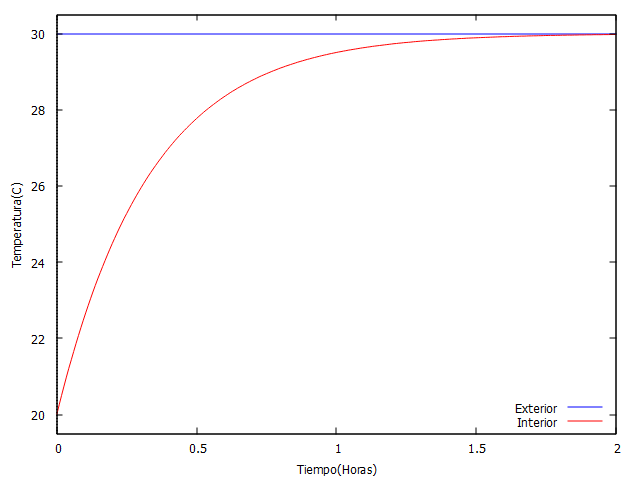
\includegraphics[width=0.7\textwidth]{grafica_ej1_tempconstante}
		\caption{Variación de la temperatura manteniendo la temperatura exterior constante}
		\label{fig:constante1}
	\end{figure}
\end{ejemplo}

\begin{ejemplo}
	Determinar la temperatura del edificio $T(t)$ si la razón de calentamiento adicional $H(t)$ es igual a la constante $H_0$, no hay calentamiento ni enfriamiento $(U(t) = 0)$ y la temperatura exterior $M$ varía como una onda senoidal en un periodo de 24 horas, con un mínimo en $t = 0$ (medianoche) y un máximo en $t = 12$ (mediodía). Es decir, 
	\begin{equation}
		M(t) = M_0 - B \cos \omega t,
	\end{equation}
	donde $B$ es una constante positiva, $M_0$ es la temperatura exterior promedio y $\omega = 2\pi /24 =\pi /12$ radianes/hora. (Esto podría ocurrir durante la primavera o el otoño cuando no hay calefactor ni aire acondicionado).\\
	\textbf{Solución.} La función $Q(t)$ que vimos en~\eqref{eq:apli1} ahora es
	\begin{equation}
		Q(t) = K(M_0 - B \cos \omega t) + H_0.
	\end{equation}
	Al hacer $B_0 := M_0 + H_0/K$, podemos escribir $Q$ como
	\begin{equation}
		Q(t) = K(B_0 - B \cos \omega t),
	\end{equation}
	donde $KB_0$ representa el valor promedio diario de $Q(t)$, es decir,
	\begin{equation}
		KB_0 = \dfrac{1}{24}\int_{0}^{24}Q(t)dt.
	\end{equation}
	Cuando la función de forzamiento $Q(t)$ que hemos obtenido se sustituye en la expresión para la temperatura en la ecuación~\eqref{eq:apli2}, el resultado, después de integrar por partes, es
	\begin{equation}
		T(t) = e^{-Kt}[\int e^{Kt}(KB_0 - KB \cos \omega t)dt + C]
	\end{equation}
	\begin{equation}\label{eq:apli3}
		T(t) = B_0 - BF(t) + Ce^{-Kt},
	\end{equation}
	donde
	\begin{equation}
		F(t) := \dfrac{\cos \omega t + (\omega / K) \sin \omega t}{1 + (\omega /K)^2}
	\end{equation}
	Elegimos la constante $C$ de modo que en medianoche $(t=0)$, el valor de temperatura $T$ sea igual a cierta temperatura inicial $T_0$. Así,
	\begin{equation}
		C = T_0 - B_0 + BF(0) = T_0 - B_0 + \dfrac{B}{1 + (\omega /K)^2}.
	\end{equation}
	Observamos que el tercer término de la solución~\eqref{eq:apli3} que multiplica a la constante $C$ tiende a cero exponencialmente. El término constante $B_0$ es igual a $M_0 + H_0/K$y representa la temperatura promedio diaria dentro del edificio (despreciando el término exponencial). Cuando no hay una razón de calentamiento adicional dentro del edificio $(H_0 = 0)$, esta temperatura promedio es igual a la temperatura exterior promedio $M_0$. El término $BF(t)$ representa la variación senoidal de la temperatura dentro del edificio correspondiente a la variación de la temperatura en el exterior.
	
	Como $F(t)$ se puede escribir en la forma
	\begin{equation}
		F(t) = [1 + (\omega /K)^2]^{-1/2}\cos (\omega t - \phi),
	\end{equation}
	donde $\tan \phi = \omega /K$, la variación senoidal dentro del edificio se retrasa con respecto de la variación en el exterior por $\phi / \omega$ horas. Además, la magnitud de la variación dentro del edificio es ligeramente menor, por un factor de $[1 + (\omega /K)^2]^{-1/2}$, que la variación en el exterior. La frecuencia angular de variación $\omega$ es $2 \pi / 24$ radianes/hora (aproximadamente $1/4$). Los valores usuales para la razón adimensional $\omega /K$ están entre $1/2$ y $1$. Para este rango, el retraso entre la temperatura interior y la exterior es aproximadamente de $1.8$ a $3$ horas y la magnitud de la variación interior está entre $89$ y $71\%$ de la variación en el exterior.
	\begin{figure}[h!]
		\centering
		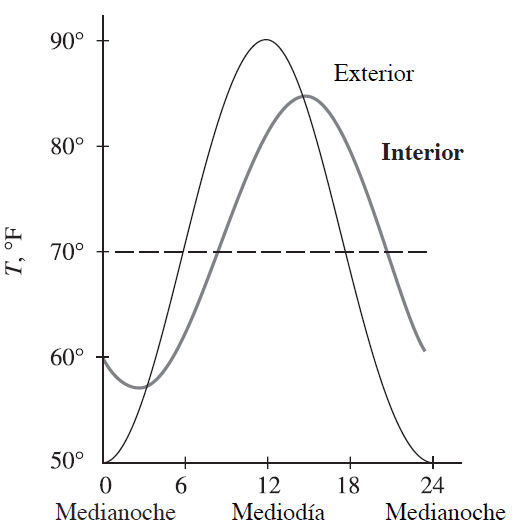
\includegraphics[width=0.7\textwidth]{fig_aplicacion1}
		\caption{Variación de la temperatura dentro y fuera de un edificio sin calefacción}
		\label{fig:aplicacion1}
	\end{figure}
	En la \autoref{fig:aplicacion1} podemos ver la variación senoidal de 24 horas de la temperatura exterior para un día moderado típico así como las variaciones de temperatura dentro del edificio para una razón adimensional $\omega /K$ de la unidad, que corresponde a una constante de tiempo $1/K$ de aproximadamente 4 horas. Los valores que hemos tomado para realizar este ejemplo concreto son:
	\begin{itemize}
		\item $M_0 = 10\celsius$ (Temperatura exterior promedio)
		\item $T_0 = 10\celsius$ (Temperatura interior inicial)
		\item $K = 0.4$
		\item $B = 4$
	\end{itemize}
	Podemos ver cómo la temperatura interior del edificio sigue el comportamiento esperado, es decir, disminuye cuando es mayor que la exterior, y viceversa, y además, a mayor es la distancia entre ambas temperaturas, mayor es la variación de la temperatura interior del edificio, como es natural.
	Al trazar esta última curva, hemos supuesto que el término exponencial ha desaparecido.
\end{ejemplo}
\section{Ejemplo con dos habitaciones}
Ahora consideremos el mismo problema con dos zonas, de modo que el calor se transfiere de una a otra en función de la diferencia de temperatura. Suponemos además que alguna de las zonas posee una fuente de calor (o de enfriamiento) que hará que ésta se caliente (o enfríe) en función de su capacidad calorífica. La variación de temperatura en cada zona será la suma del calor (o frío) generado por dicha fuente, si existe en esa zona, y la pérdida o ganancia de calor generada por el contacto con otras zonas o con el exterior. Para calcular las ecuaciones aplicaremos la \textit{ley de Newton del enfriamiento} vista anteriormente.
\begin{ejemplo}
	Un estudio consta de dos zonas: la zona A de la planta alta y la zona B de la planta baja como podemos ver en la \autoref{fig:aplicacion2}. La planta baja, que tiene una capacidad calorífica de $(1/5)\degree C /1000$ btu (btu: unidades térmicas británicas), es calentada por un calefactor que genera $90000$ btu por hora. Las constantes de tiempo de transferencia de calor son: $3$ horas entre la planta baja y el exterior, $1/2$ hora entre la planta alta y el exterior y $1/2$ hora entre las dos plantas. Si la temperatura en el exterior permanece constante a $2\degree C$ e inicialmente ambas zonas estaban a $22\degree C$, calculemos la temperatura en la planta baja al cabo de $1$ hora.
	
	\begin{figure}[h!]
		\centering
		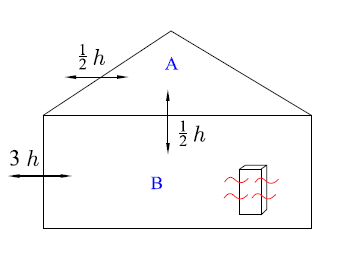
\includegraphics[width=0.6\textwidth]{aplicacion2}
		\caption{Calentamiento de edificio compuesto por dos zonas.}
		\label{fig:aplicacion2}
	\end{figure}
	\textbf{Solución.} En este caso, tenemos tres regiones, la zona A, la zona B y el exterior, luego tendremos que tener en cuenta la transferencia de calor entre
	las tres.
	
	Sea $x(t)$ la temperatura en la zona $A$ en un instante $t$ y sea $y(t)$ la temperatura en la zona $B$ en un instante $t$.
	
	La zona B recibe el calor generado por el calefactor a razón de $90000 btu/h$, puesto que su capacidad calorífica es de  $(1/5)\degree C /1000$ btu, tendremos que la temperatura que gana $B$ es:
	\begin{equation}
		90000 btu/h \times (1/5)\degree C /1000 btu = 18\degree C/h.
	\end{equation}
	La variación de temperatura en las zonas $A$ y $B$ vendrá dada por:
	\begin{equation}
		\dfrac{dx}{dt} = 2(2-x)+2(y-x)
	\end{equation}
	\begin{equation}
		\dfrac{dy}{dt} = \dfrac{1}{3}(2-y)+2(x-y) + 18.
	\end{equation}
	Por tanto, tenemos el sistema no homogéneo:
		\begin{equation}
		\dfrac{dx}{dt} = -4x+2y-4
	\end{equation}
	\begin{equation}
		\dfrac{dy}{dt} = 2x-\dfrac{7}{3}y+\dfrac{56}{3}
	\end{equation}
	Resolvamos el sistema. La ecuación característica es:
	\begin{equation}
		\begin{vmatrix} -4-r & 2 \\ 2 & -\dfrac{7}{3}-r \end{vmatrix} = 0 \rightarrow 3r^2 + 19r + 16 =0,
	\end{equation}
	cuyas raíces son los valores propios: $r_1 = -1 y r_2 = -\dfrac{16}{3}$. Calculemos los vectores propios asociados a cada valor:
	\begin{equation}
		H_{-1} = \{(x,y): \begin{pmatrix}
			-3 & 2\\ 
			2 & -\dfrac{4}{3} 
		\end{pmatrix} \begin{pmatrix}
		x \\ 
		y
		\end{pmatrix} = \begin{pmatrix}
		0 \\ 
		0  
		\end{pmatrix}\} = \{(x,y): -3x + 2y = 0\},
	\end{equation}
	\begin{equation}
		H_{-16/3} = \{(x,y): \begin{pmatrix}
			\dfrac{4}{3} & 2\\ 
			2 & 3
		\end{pmatrix} \begin{pmatrix}
			x \\ 
			y
		\end{pmatrix} = \begin{pmatrix}
			0 \\ 
			0  
		\end{pmatrix}\} = \{(x,y): 2x + 3y = 0\},
	\end{equation}
	Por tanto, un vector propio asociado a $r_1 = -1$ es $\vec{u}_1 = \begin{pmatrix}
		2 \\ 
		3
	\end{pmatrix}$ y un vector propio asociado a $r_2 = -\dfrac{16}{3}$ es $\vec{u}_2 = \begin{pmatrix}
	3 \\ 
	-2
	\end{pmatrix}$ y la solución de la parte homogénea resulta:
	\begin{equation}
		\vec{x}_h(t) = \begin{pmatrix}	x_h(t) \\ y_h(t)	\end{pmatrix} = C_1e^{-t}\begin{pmatrix}	2 \\ 3	\end{pmatrix} + C_2e^{-16t/3}\begin{pmatrix}	3 \\ -2	\end{pmatrix}.
	\end{equation}
	Ahora buscamos una solución particular mediante el método de los coeficientes
	indeterminados. Puesto que el término no homogéneo es un polinomio de grado
	$0$ y además $0$ no es raíz de la ecuación característica, podemos tomar la solución particular de la forma:
	\begin{equation}
		\vec{x}_p = \vec{a} = \begin{pmatrix}	a_1 \\ a_2	\end{pmatrix}.
	\end{equation}
	Derivando y sustituyendo en la ecuación, tenemos:
	\begin{equation}
		\begin{pmatrix}	0 \\ 0	\end{pmatrix} = \begin{pmatrix}
		    -4 & 2\\ 
			2 & -\dfrac{7}{3}
		\end{pmatrix} \begin{pmatrix}	a_1 \\ a_2	\end{pmatrix} +  \begin{pmatrix}	4 \\ 56/3	\end{pmatrix}
	\end{equation}
	pasando el término independiente al otro lado de la igualdad,
	\begin{equation}
		\begin{pmatrix}
			-4 & 2\\ 
			2 & -\dfrac{7}{3}
		\end{pmatrix}\begin{pmatrix}	a_1 \\ a_2	\end{pmatrix} = \begin{pmatrix}	-4 \\ -	56/3\end{pmatrix}
	\end{equation}
	de donde obtenemos: $a_1 = 35/4$ y $a_2 = 31/2.$ La solución general es:
	\begin{equation}
		\vec{x}(t) = \begin{pmatrix}	x(t) \\ y(t)	\end{pmatrix} = C_1e^{-t}\begin{pmatrix}	2 \\ 3	\end{pmatrix} + C_2e^{-16t/3}\begin{pmatrix}	3 \\ -2	\end{pmatrix} + \begin{pmatrix}	35/4 \\ 31/2	\end{pmatrix}
	\end{equation}
	Considerando las condiciones iniciales: para $t=0, x(0) = 22$ y $y(0) = 22$, se tiene:
	\begin{equation}
		\begin{pmatrix}	22 \\ 22	\end{pmatrix} = C_1 \begin{pmatrix}	2 \\ 3	\end{pmatrix} + C_2 \begin{pmatrix}	3 \\ -2	\end{pmatrix} + \begin{pmatrix}	35/4 \\ 31/2	\end{pmatrix}
	\end{equation}
	Agrupando los términos independientes y reescribiendo los sumandos multiplicados
	por las constantes $C_1$ y $C_2$ en términos de la matriz fundamental, tenemos:
	\begin{equation}
		\begin{pmatrix}
			2 & 3\\ 
			3 & -2
		\end{pmatrix}\begin{pmatrix}	C_1 \\ C_2	\end{pmatrix} = \begin{pmatrix}	53/4 \\ 13/2	\end{pmatrix}
	\end{equation}
	y resolviendo el sistema obtenemos:
	\begin{equation}
		C_1 = 46/13 \qquad y \qquad C_2 = 107/52.
	\end{equation}
	La solución a este problema de valor inicial es:
	\begin{equation}
		\vec{x}(t) = \begin{pmatrix}	x(t) \\ y(t)	\end{pmatrix} = \dfrac{46}{13}e^{-t}\begin{pmatrix}	2 \\ 3	\end{pmatrix} + \dfrac{107}{52}e^{-16t/3}\begin{pmatrix}	3 \\ -2	\end{pmatrix} + \begin{pmatrix}	35/4 \\ 31/2	\end{pmatrix}.
	\end{equation}
	Puesto que la temperatura en $B$ era $y(t)$, ésta al cabo de $1h$ será:
	\begin{equation}
		y(1) = \dfrac{46}{13}e^{-t}3 + \dfrac{107}{52}e^{-16t/3}(-2) + \dfrac{31}{2} \approx 19,405\degree C.
	\end{equation}
\end{ejemplo}

\section{Modelo de un edificio con 5 habitaciones}
Temperatura en A -> a(t)
B -> b(t)
C -> c(t)
D -> d(t)
E -> e(t)
F -> M(t)
Constante de transferencia entre espacio -> K
Calor generado por cada aire acondicionado en la habitación B -> U\_B(t)
Calor generado por cada aire acondicionado en la habitación D -> U\_D(t)
Calor generado en el interior -> H(t)
\begin{equation}\begin{dcases}
	 \dfrac{\partial}{\partial t}a(t)= \dfrac{b(t)-a(t)}{K_{AB}} + \dfrac{M(t) - a(t)}{K_{AF}} \\  \dfrac{\partial}{\partial t}b(t)= \dfrac{a(t)-b(t)}{K_{AB}} + \dfrac{c(t)-b(t)}{K_{BC}} + \dfrac{M(t) - b(t)}{K_{BF}} + U_B(t) \\  \dfrac{\partial}{\partial t}c(t)= \dfrac{b(t)-c(t)}{K_{BC}} + \dfrac{d(t)-c(t)}{K_{CD}} + \dfrac{M(t) - c(t)}{K_{CF}} \\  \dfrac{\partial}{\partial t}d(t)= \dfrac{c(t)-d(t)}{K_{CD}} + \dfrac{e(t)-d(t)}{K_{DE}} + \dfrac{M(t) - d(t)}{K_{DF}} + U_D(t) \\  \dfrac{\partial}{\partial t}e(t)= \dfrac{d(t)-e(t)}{K_{DE}} + \dfrac{M(t) - e(t)}{K_{EF}} \end{dcases}
\end{equation}
\begin{figure}[h!]
	\centering
	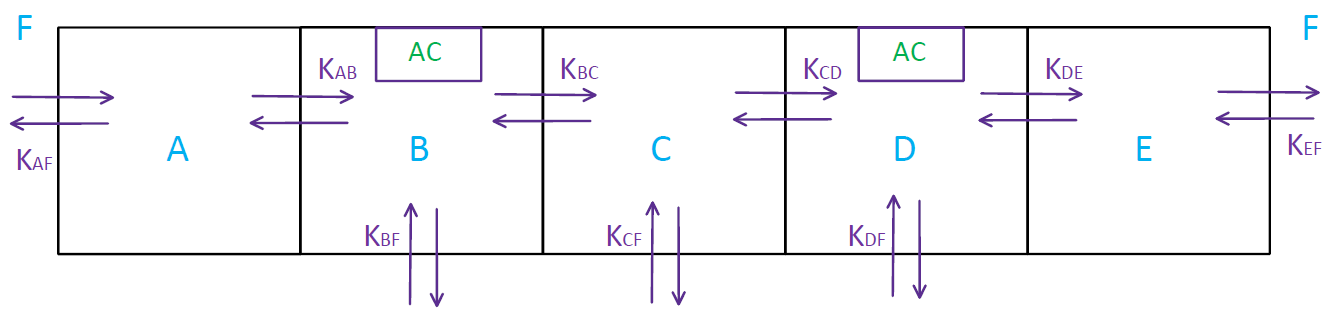
\includegraphics[width=\textwidth]{edificio_5habs}
	\caption{Edificio con 5 habitaciones contiguas}
	\label{fig:edif5}
\end{figure}


\endinput
%------------------------------------------------------------------------------------
% FIN DEL CAPÍTULO. 
%----------------------------------------------------------------------------------
-

% --------------------------------------------------------------------
% APPENDIX: Opcional
% --------------------------------------------------------------------

\appendix % Reinicia la numeración de los capítulos y usa letras para numerarlos
\pdfbookmark[-1]{Apéndices}{appendix} % Alternativamente podemos agrupar los apéndices con un nuevo \part{Apéndices}

% !TeX root = ../libro.tex
% !TeX encoding = utf8

\chapter{Primer apéndice}\label{ap:apendice1}

Los apéndices son opcionales.

Archivo: \texttt{apendices/apendice01.tex}

\endinput
%------------------------------------------------------------------------------------
% FIN DEL APÉNDICE. 
%------------------------------------------------------------------------------------

% Añadir tantos apéndices como sea necesario 

% --------------------------------------------------------------------
% GLOSARIO: Opcional
% --------------------------------------------------------------------

% !TeX root = ../libro.tex
% !TeX encoding = utf8

\chapter*{Glosario}
\addcontentsline{toc}{chapter}{Glosario} % Añade el glosario a la tabla de contenidos

La inclusión de un glosario es opcional.

Archivo: \texttt{glosario.tex}

\begin{description} 
  \item[$\mathbb{R}$] Conjunto de números reales.

  \item[$\mathbb{C}$] Conjunto de números complejos.

  \item[$\mathbb{Z}$] Conjunto de números enteros.
\end{description}
\endinput
 

% -------------------------------------------------------------------
% BACKMATTER
% -------------------------------------------------------------------

\backmatter % Desactiva la numeración de los capítulos
\pdfbookmark[-1]{Referencias e Índices}{BM-Referencias}

% BIBLIOGRAFÍA
%-------------------------------------------------------------------

\setbibpreamble{Las referencias se listan por orden alfabético. Aquellas referencias con más de un autor están ordenadas de acuerdo con el primer autor.\par\bigskip}
\bibliographystyle{alpha} 
\begin{small} % Normalmente la bibliografía se imprime en un tamaño de letra más pequeño.
\bibliography{library.bib}
\end{small}


% ÍNDICE TERMINOLÓGICO  (Opcional) 
%------------------------------------------------------------------- 

% Para incluir el índice terminológico es necesario descomentar los siguientes comandos. Incluir un índice terminológico es opcional

% \cleardoublepage 
% \begin{footnotesize} % Normalmente el índice se imprime en un tamaño de letra más pequeño.
% \printindex 
% \end{footnotesize}

\end{document}
